%  article.tex (Version 3.3, released 19 January 2008)
%  Article to demonstrate format for SPIE Proceedings
%  Special instructions are included in this file after the
%  symbol %>>>>
%  Numerous commands are commented out, but included to show how
%  to effect various options, e.g., to print page numbers, etc.
%  This LaTeX source file is composed for LaTeX2e.

%  The following commands have been added in the SPIE class 
%  file (spie.cls) and will not be understood in other classes:
%  \supit{}, \authorinfo{}, \skiplinehalf, \keywords{}
%  The bibliography style file is called spiebib.bst, 
%  which replaces the standard style unstr.bst.  

\documentclass[]{spie}  %>>> use for US letter paper
%%\documentclass[a4paper]{spie}  %>>> use this instead for A4 paper
%%\documentclass[nocompress]{spie}  %>>> to avoid compression of citations
%% \addtolength{\voffset}{9mm}   %>>> moves text field down
%% \renewcommand{\baselinestretch}{1.65}   %>>> 1.65 for double spacing, 1.25 for 1.5 spacing 
%  The following command loads a graphics package to include images 
%  in the document. It may be necessary to specify a DVI driver option,
%  e.g., [dvips], but that may be inappropriate for some LaTeX 
%  installations. 
\usepackage[]{graphicx}
\usepackage{amsmath}

\title{The ANTs cortical thickness processing pipeline} 

%>>>> The author is responsible for formatting the 
%  author list and their institutions.  Use  \skiplinehalf 
%  to separate author list from addresses and between each address.
%  The correspondence between each author and his/her address
%  can be indicated with a superscript in italics, 
%  which is easily obtained with \supit{}.

\author{Nicholas J. Tustison\supit{a}, Brian B. Avants\supit{b}, Philip A. Cook\supit{b}, Gang Song\supit{b}, Sandhitsu Das\supit{b}, Niels van Strien\supit{c}, James R. Stone\supit{a}, James C. Gee\supit{b}
\skiplinehalf
\supit{a}Dept. of Radiology and Medical Imaging, Univ. of Virginia, Charlottesville, Virginia, USA\\
\supit{b}PICSL, Univ. of Pennsylvania, Philadelphia, Pennsylvania, USA\\
\supit{c}Dept. of Circulation and Medical Imaging, Norwegian University of Science and Technology, Trondheim, Norway\\
}

%>>>> Further information about the authors, other than their 
%  institution and addresses, should be included as a footnote, 
%  which is facilitated by the \authorinfo{} command.

\authorinfo{Further author information: (Send correspondence to N.J.T.)\\
            N.J.T.: E-mail: njt4n@virginia.edu, Telephone: 1 434 924 7730}
%%>>>> when using amstex, you need to use @@ instead of @
 

%%%%%%%%%%%%%%%%%%%%%%%%%%%%%%%%%%%%%%%%%%%%%%%%%%%%%%%%%%%%% 
%>>>> uncomment following for page numbers
% \pagestyle{plain}    
%>>>> uncomment following to start page numbering at 301 
%\setcounter{page}{301} 
 
  \begin{document} 
  \maketitle 

%%%%%%%%%%%%%%%%%%%%%%%%%%%%%%%%%%%%%%%%%%%%%%%%%%%%%%%%%%%%% 
\begin{abstract}
Numerous studies have explored the relationship between cortical
structure and brain development, cognitive 
function, and functional connectivity.
The highly convoluted cortical topography makes manual measurements
arduous and often impractical given the population sizes necessary 
for sufficient statistical power.  Computational techniques 
have permitted large-scale studies as they
provide robust and reliable localized measurements characterizing
the cortex with little or no human intervention.  Particularly useful
to the neuroscience community are publicly available tools, such as the popular 
surface-based Freesurfer, which facilitate the testing and refinement of 
hypotheses.  In this paper, we introduce the volume-based 
Advanced Normalization Tools
(ANTs) cortical thickness automated pipeline
comprising well-vetted components such as SyGN (multivariate template construction),
SyN (image registration), N4 (bias
correction),
Atropos ($n$-tissue segmentation), and DiReCT (cortical thickness) 
all developed as part of the ANTs open science effort.  
Complementing the open source aspect of ANTs we demonstrate its
utility using the publicly available IXI data set.
\end{abstract}

%>>>> Include a list of keywords after the abstract 

\keywords{advanced normalization tools, DiReCT, Insight Toolkit, KellyKapowski}

%%%%%%%%%%%%%%%%%%%%%%%%%%%%%%%%%%%%%%%%%%%%%%%%%%%%%%%%%%%%%
\section{INTRODUCTION}
\label{sec:intro}  % \label{} allows reference to this section

Historically rooted in the meticulous work of von Economo \cite{economo2008},
imaging-based structural analysis of the brain plays a fundamental role
in identifying the relationship between cortical morphology, disease and cognition.
The availability of quantitative computational methods for extracting such information
has proven invaluable for developing and refining fundamental 
neuroscience hypotheses.  Computational methods for analyzing the cortex may be 
broadly characterized as surface mesh-based or volumetric.  
Representative of the former is the
Freesurfer%
\footnote{
http://surfer.nmr.mgh.harvard.edu/
}
cortical modeling software package \cite{dale1999,fischl1999}.
%which owes its popularity to public availability, excellent documentation, 
%good performance, and  integration with other toolkits.  
Similar to other surface
approaches, the pial
and white matter surfaces from individual subject MR data are modeled with polygonal meshes  
which are then used to determine local cortical thickness based on a specified correspondence between 
the surface models.
In contrast, volumetric approaches directly operate in the image space.  For example, 
DiReCT (Diffeomorphic Registration-based 
Cortical Thickness) algorithm\cite{das2009} is 
a registration-based approach where the derived diffeomorphic mapping between the 
white and pial matter surfaces is used to propagate thickness values 
through the cortical gray matter.  
%A unique benefit of DiReCT is that it
%naturally estimates the boundaries of buried sulci by employing a
%diffeomorphic constraint on the probabilistic estimate of the gray
%matter and cerebrospinal fluid interface.  

Despite the variety of techniques for estimating cortical thickness
from imaging data, several common pre-processing components
can be identified.
The most fundamental of these include inhomogeneity correction, skull stripping, and $n$-tissue segmentation 
for differentiating the gray and white matter. 
In this work, we describe our C$++$ based cortical thickness pipeline
which is freely available as part of the Advanced Normalization Tools
(ANTs) software package based on the Insight Toolkit.  This includes 
all the necessary preprocessing steps consisting
of well-vetted previously published algorithms for bias correction \cite{tustison2010},
brain extraction \cite{avants2010a}, $n$-tissue segmentation \cite{avants2011a},
template construction \cite{avants2010}, and image normalization \cite{avants2011}.
Equally as important, we demonstrate how to coordinate
these pipeline components and provide a set of useful parameters
which are employed to analyze the publicly available IXI data set. The
full pipeline and parameter set is 
encapsulated in a well-documented shell script which is also available in ANTs. 


%%%%%%%%%%%%%%%%%%%%%%%%%%%%%%%%%%%%%%%%%%%%%%%%%%%%%%%%%%%%%
\section{MATERIALS AND METHODS} 

\begin{figure}
  \centering
  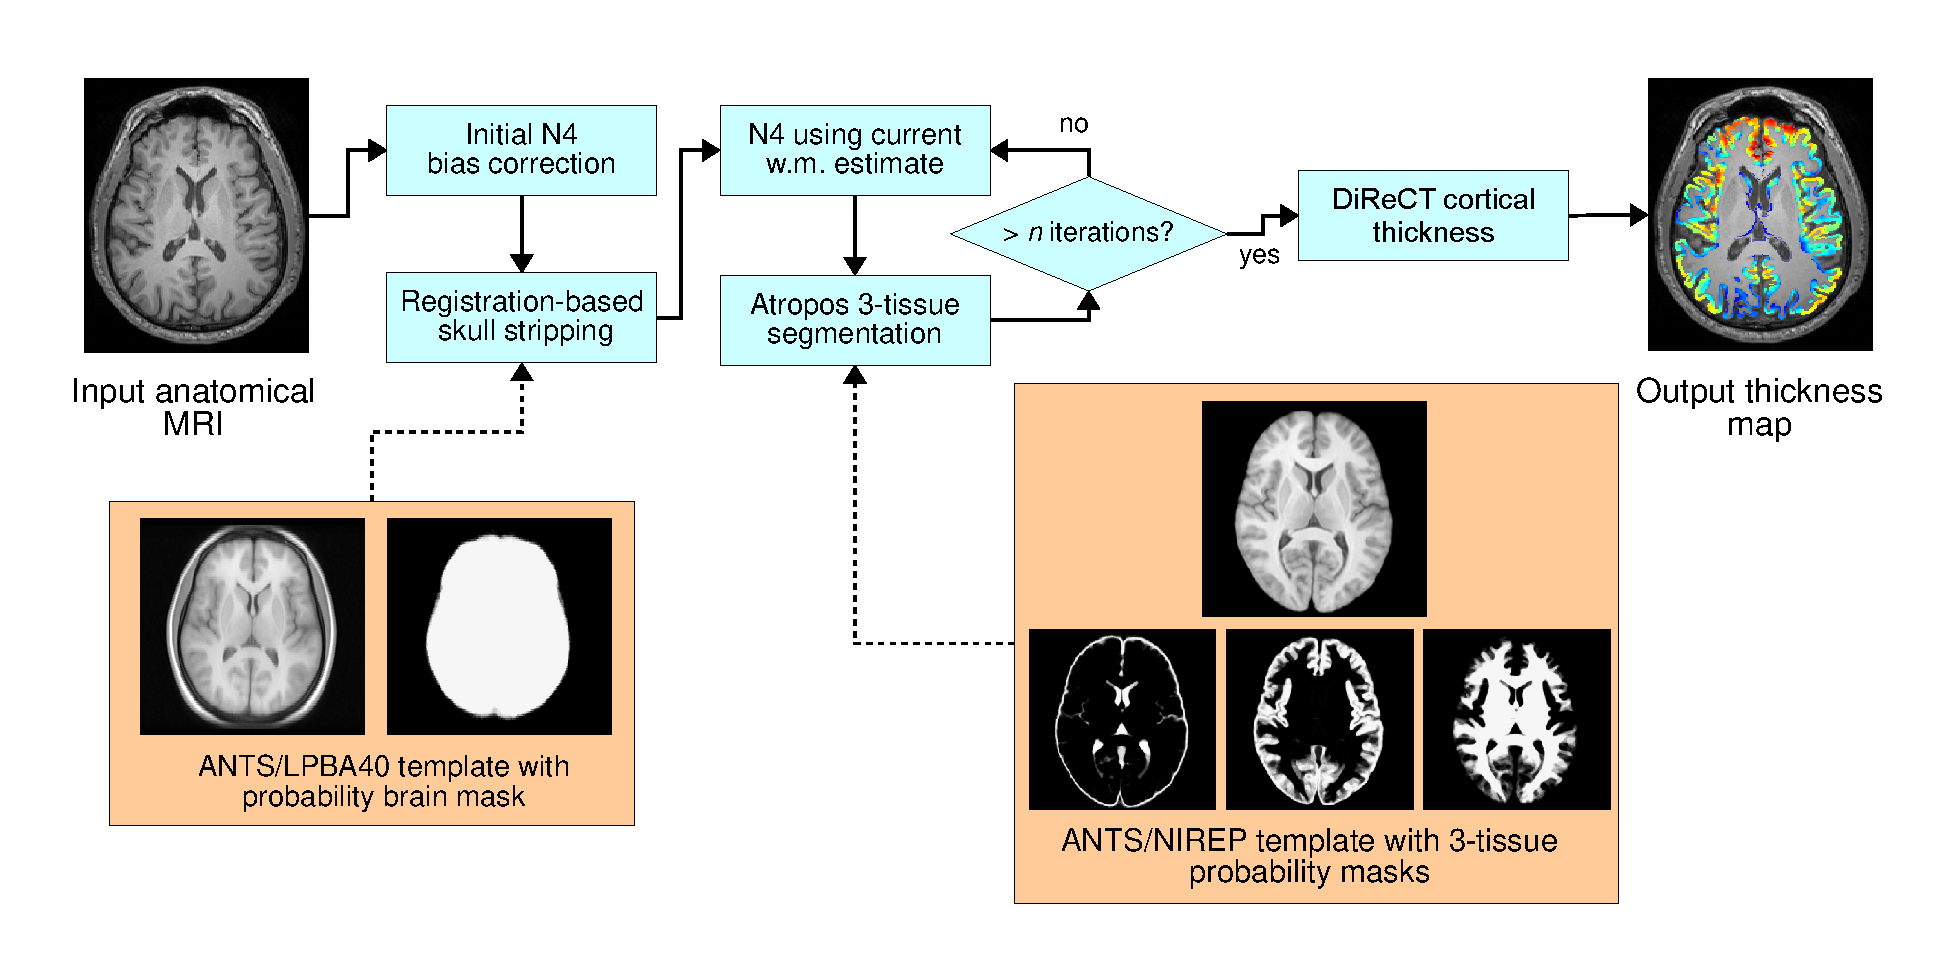
\includegraphics[width=120mm]{Kapowski_pipeline2.pdf}
  \caption{The ANTs T1 processing workflow containing all elements for 
  determining cortical thickness.   
  Not shown is the optional single subject
  to template registration.
  }
  \label{fig:pipeline}
\end{figure}

The ANTs-based cortical thickness estimation workflow is illustrated 
in Figure \ref{fig:pipeline}.  The steps are as follows: 
1) initial N4 bias correction on input anatomical MRI,
2) brain extraction using a hybrid segmentation/template-based strategy,
3) alternating between prior-based segmentation and white matter posterior
        probability weighted bias correction,
4) DiReCT-based cortical thickness estimation, and
5) optional normalization to specified template.
The coordination of all the algorithmic components is
encapsulated in the shell script \texttt{antsCorticalThickness.sh}.  
This includes
optimal parameters for each of the algorithmic components which were used to acquire the results 
described in this work.

\subsection{Description of Processing Pipeline Components}
\begin{description}
\item[N4:] We introduced an extension of N3 into ANTs, denoted as N4, which demonstrates 
improved performance and convergence behavior on a variety of data. This improvement 
is a result of an enhanced fitting routine and a modified optimization formulation. 
For our workflow, the additional possibility of specifying a weighted mask in N4 
permits the use of the current white matter probability map calculated during the 
segmentation pipeline for further improvement of bias field estimation.
\item[Atropos:]  Our $n$-tissue segmentation
software tool (which we denote as �Atropos�) attempts to distill 20+ years of active research 
in this area particularly some of its most seminal work. Specification of prior probabilities includes spatially varying Markov Random Field modeling, prior label maps, and prior probability maps typically derived from our template building process. Additional capabilities include handling of multivariate data, partial volume modeling, a memory-minimization mode, label propagation, a plug-n-play architecture for incorporation of novel likelihood models which includes both parametric and non-parametric models for both scalar and tensorial images, and alternative posterior formulations for different segmentation tasks.
\item[Brain extraction:]  Brain extraction using ANTs combines template building, high-performance brain image registration [5], and Atropos with topological refinements. An optimal template for brain extraction is generated offline using labeled brain data. For example, in this work we use the LPBA40 data for generating a brain extraction template and a corresponding brain probability mask.  A comparison\cite{avants2010a} using open access brain data with other publicly available brain extraction algorithms demonstrated that our combined registration/segmentation approach performs at the top level alongside BrainSuite (tuned) and FreeSurfer.
\item[DiReCT:] Although the basic formulation of DiReCT as reported in this work is as it was introduced, we have made several improvements. Perhaps the most significant advance is that this particular ITK-compatible implementation has been significantly multi-threaded, is written in ITK coding style, and has been made publicly available through ANTs complete with a unique user interface design developed specifically for ANTs tools.
\end{description}

\subsection{Description of Publicly Available Image Data Sets}

Several publicly available data sets were used in this work.  The IXI data%
\footnote{
http://biomedic.doc.ic.ac.uk/brain-development/
}
were processed to produce the cortical thickness maps.  
They were also used to construct the gender/age-based
multivariate templates consisting of T1, T2, proton density,
and FA components.  
%Sample axial slices from
%the female, age 50--60 subgroup template are shown in the middle of Fig. \ref{fig:template}.
The annotated NIREP NA0%
\footnote{
http://www.nirep.org
}
and LPBA40%
\footnote{
http://www.loni.ucla.edu/Atlases/LPBA40/
}
data sets were used, respectively, in the processing pipeline for 
 3-tissue segmentation and brain extraction
for each subject (as illustrated in Fig. \ref{fig:pipeline}).  Additionally,
we registered the NIREP template to the total template to propagate the NIREP
NA0 labels for tabulating thickness values in each of the 32 cortical labels
over the male and female IXI subjects.


%\paragraph{IXI:} The IXI data set consists of approximately 600 subjects.  Demographic
%information including gender and age is also available for each subject.  Further
%details can be found on the IXI website.%
%\footnote{
%}  
%Each subject was processed using the \texttt{antsCorticalThickness} script ultimately
%yielding cortical maps for each IXI subject.  

%\begin{figure}
%  \centering
%  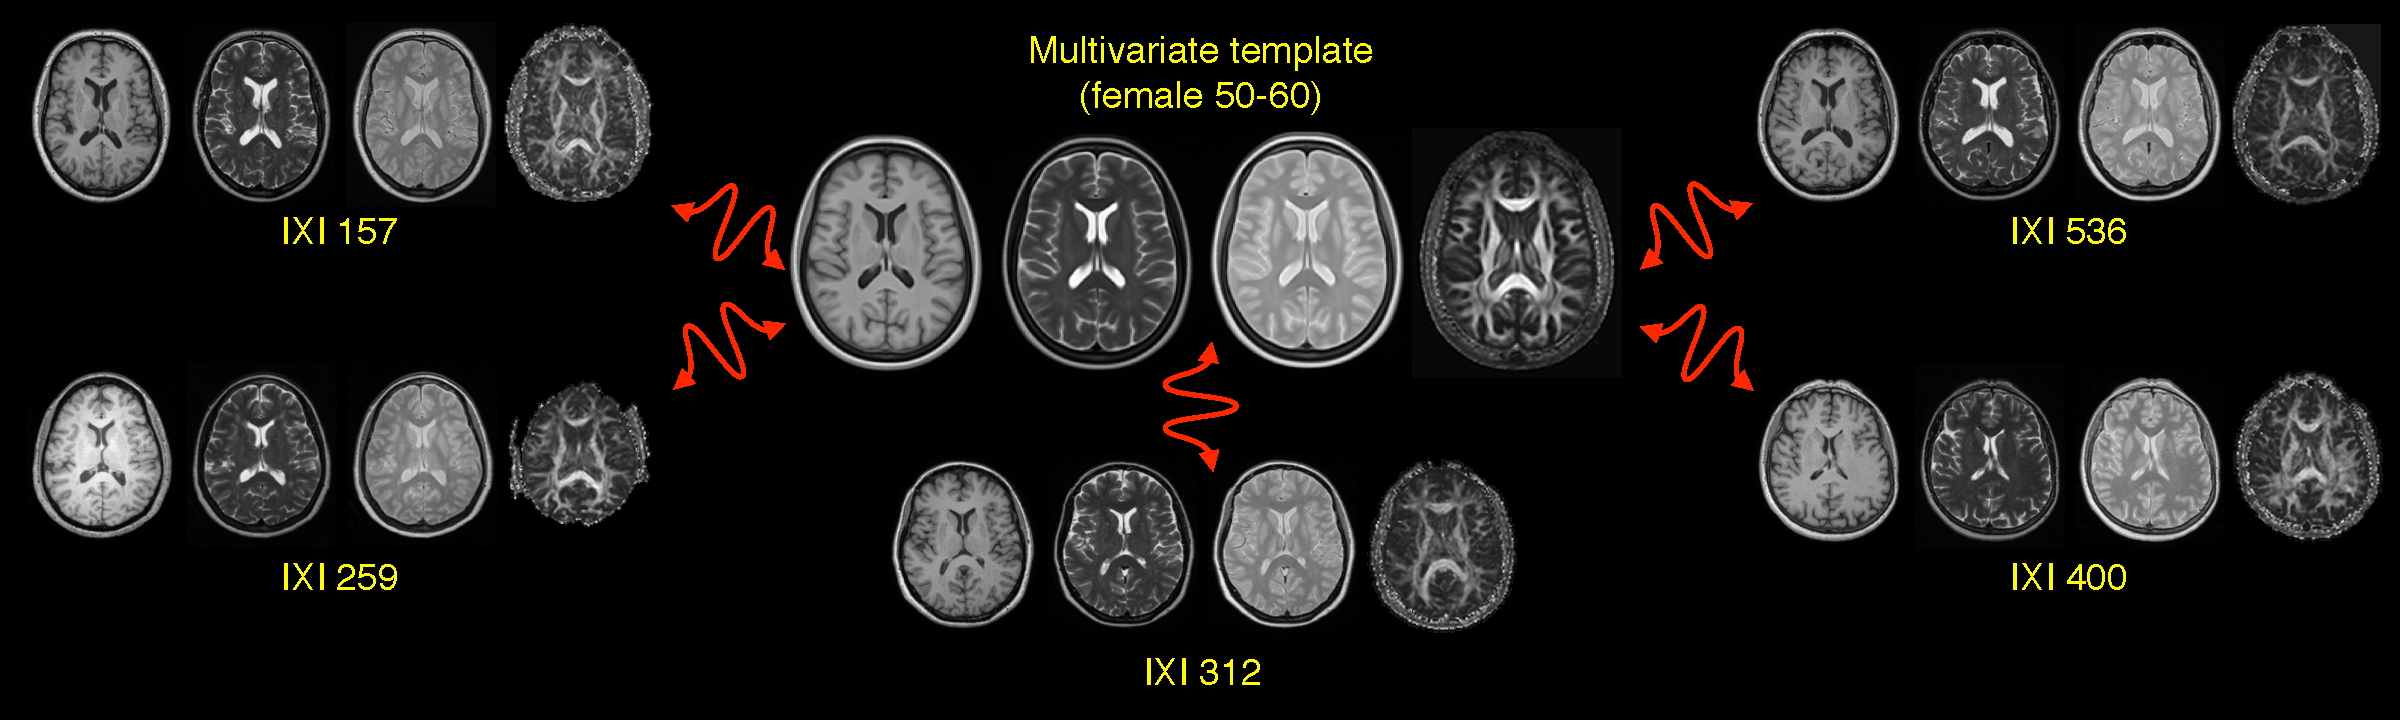
\includegraphics[width=170mm]{template50_60_long.pdf}
%  \caption{Multivariate template (T1, T2, PD, and FA) made from the IXI female, age 50--60 cohort.  
%  The set of all gender/age-based templates were then used to create a final template which
%  served as the normalized space for statistical comparison.
%  }
%  \label{fig:template}
%\end{figure}

%Age and gender-based multivariate templates\cite{avants2010} were also created from the IXI data
%consisting of T1, T2, proton-density (PD), and FA components.  Sample axial slices from
%the female, age 50--60 subgroup template are shown in the middle of Fig. \ref{fig:template}.  Each
%subject-specific set of T1, T2, PD, and FA images (of which 5 are shown) are weighted equally in constructing
%the multivariate template.


%%%%%%%%%%%%%%%%%%%%%%%%%%%%%%%%%%%%%%%%%%%%%%%%%%%%%%%%%%%%%
\section{RESULTS} 

The resulting thickness values for each subject were averaged within each
of the 32 labels subsequent to normalization of thickness values by the
ratio of the template volume to the individual subject volume.
Normalized cortical thickness plots (age vs. thickness) are given in Fig.
\ref{fig:nirep}.


%\begin{figure}
%  \centering
%  \begin{tabular}{cccc}
%  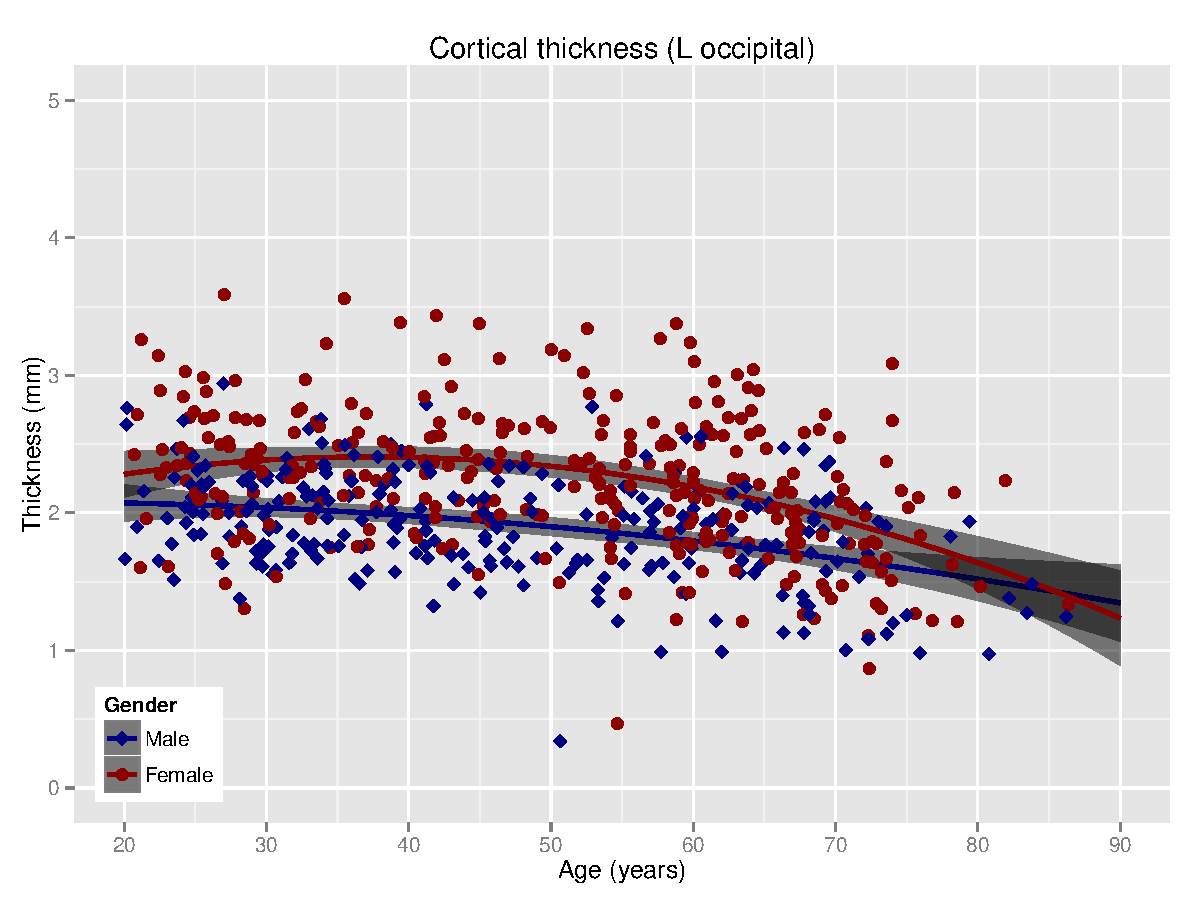
\includegraphics[width=51mm]{IXI_results/yylabel1_results.pdf} &
%  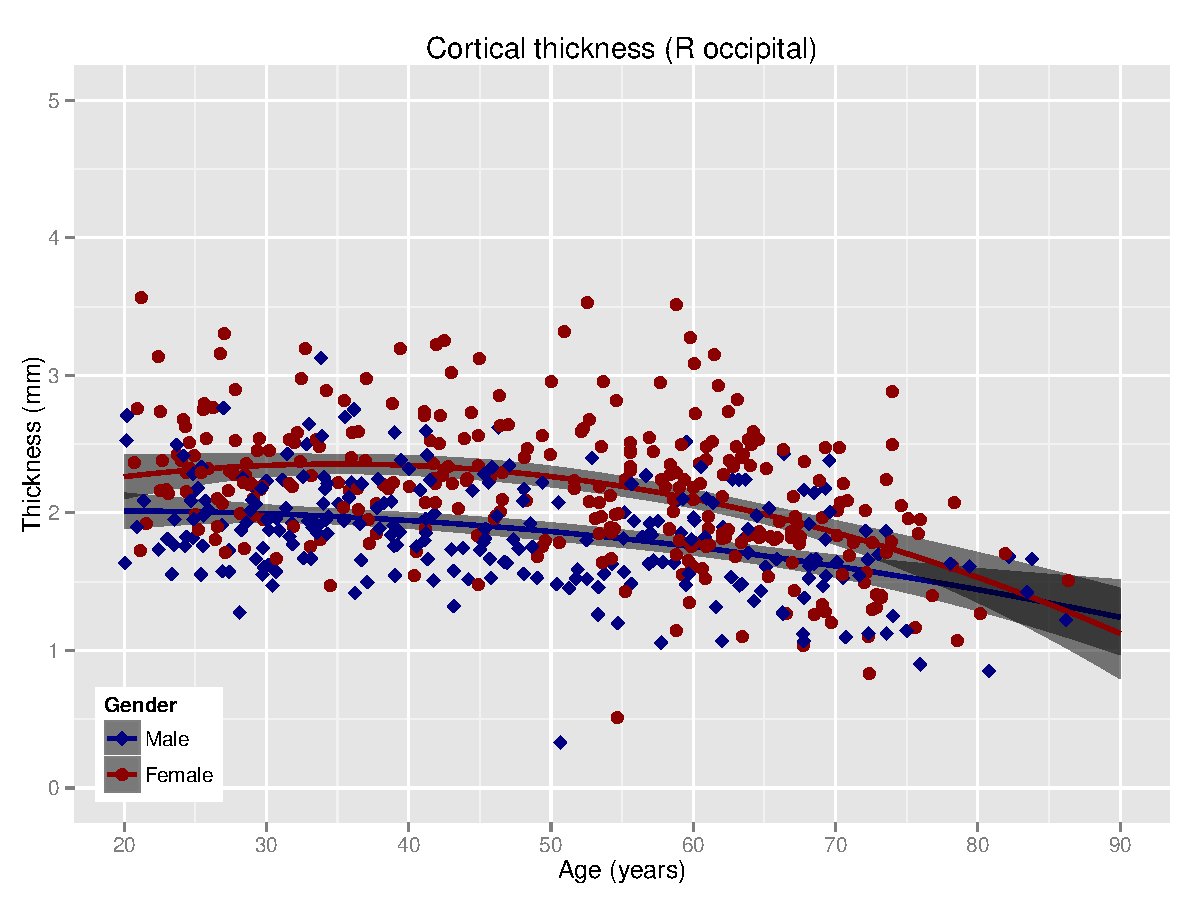
\includegraphics[width=51mm]{IXI_results/yylabel2_results.pdf} &
%  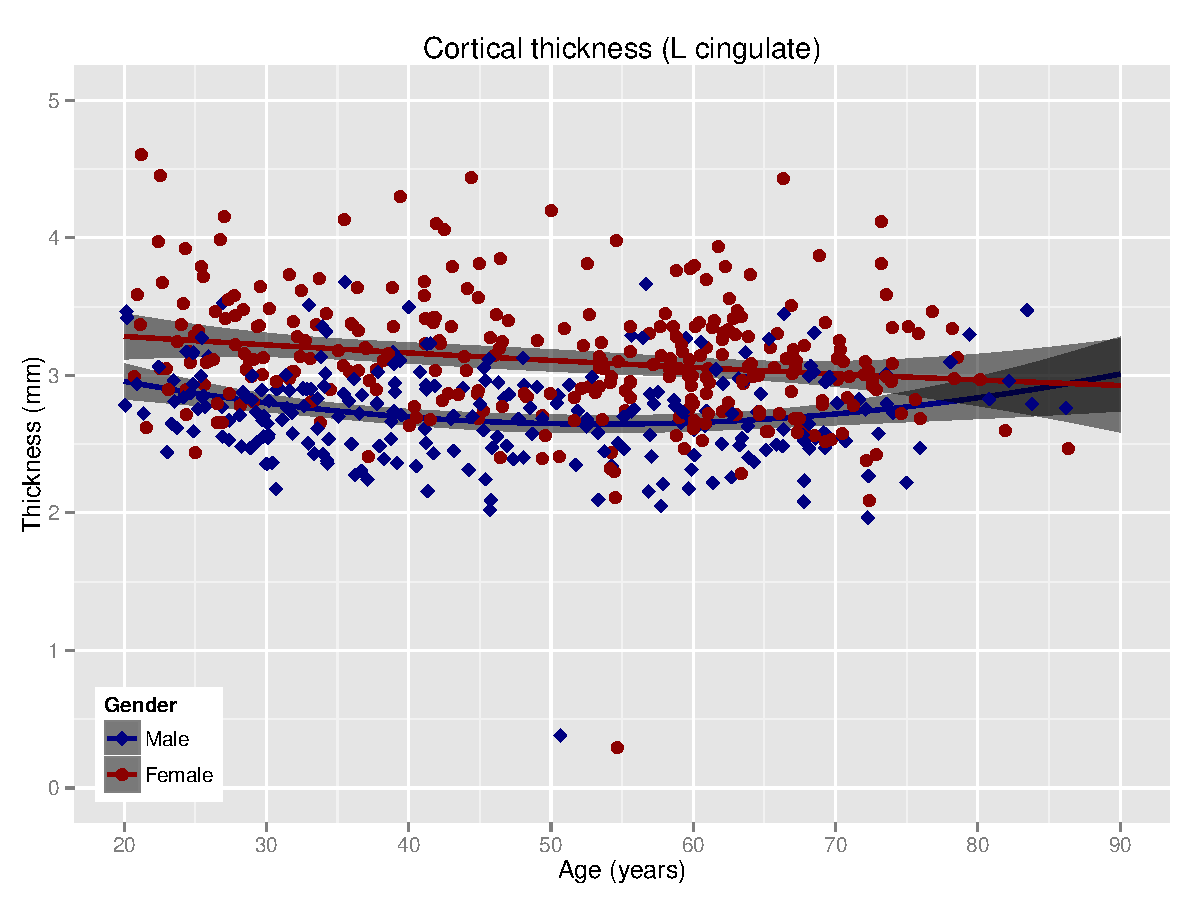
\includegraphics[width=51mm]{IXI_results/yylabel3_results.pdf} &
%  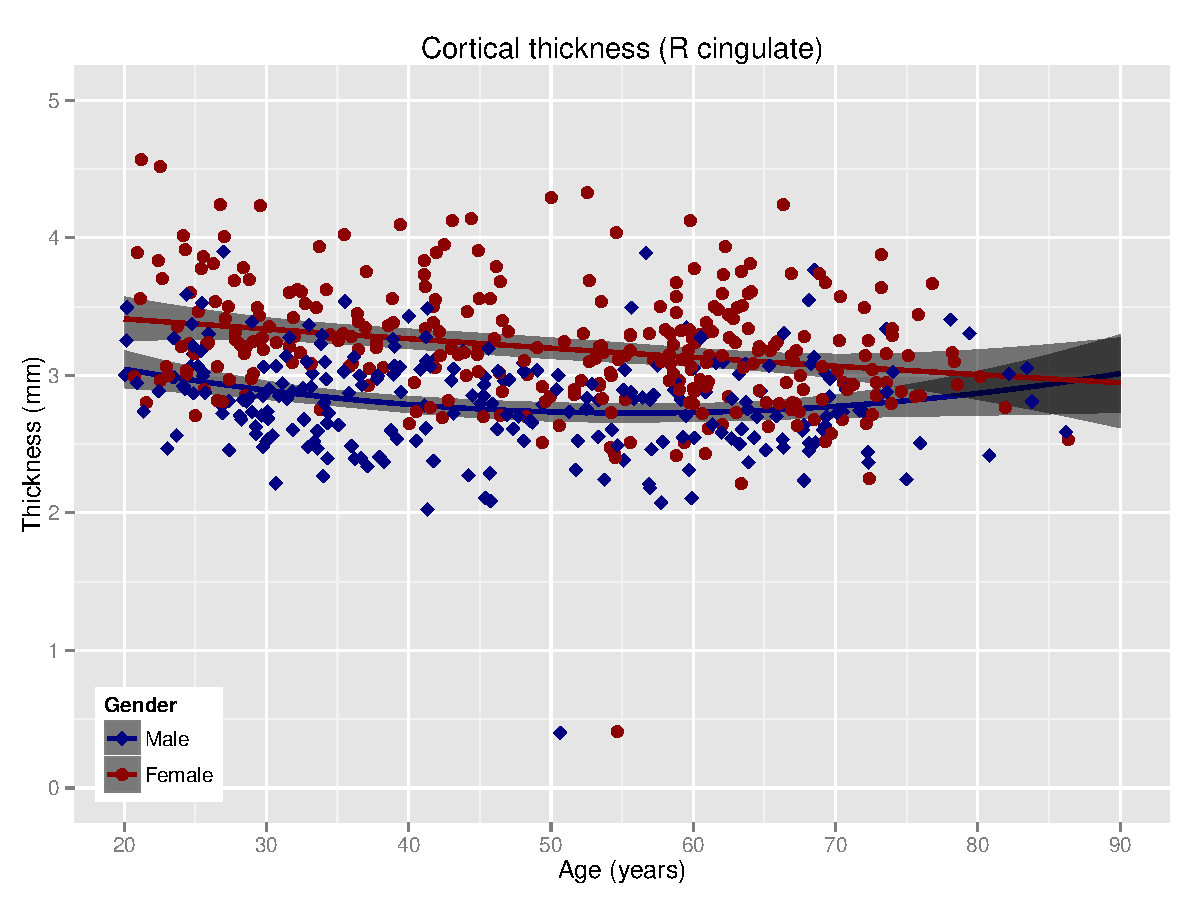
\includegraphics[width=51mm]{IXI_results/yylabel4_results.pdf} \\
%  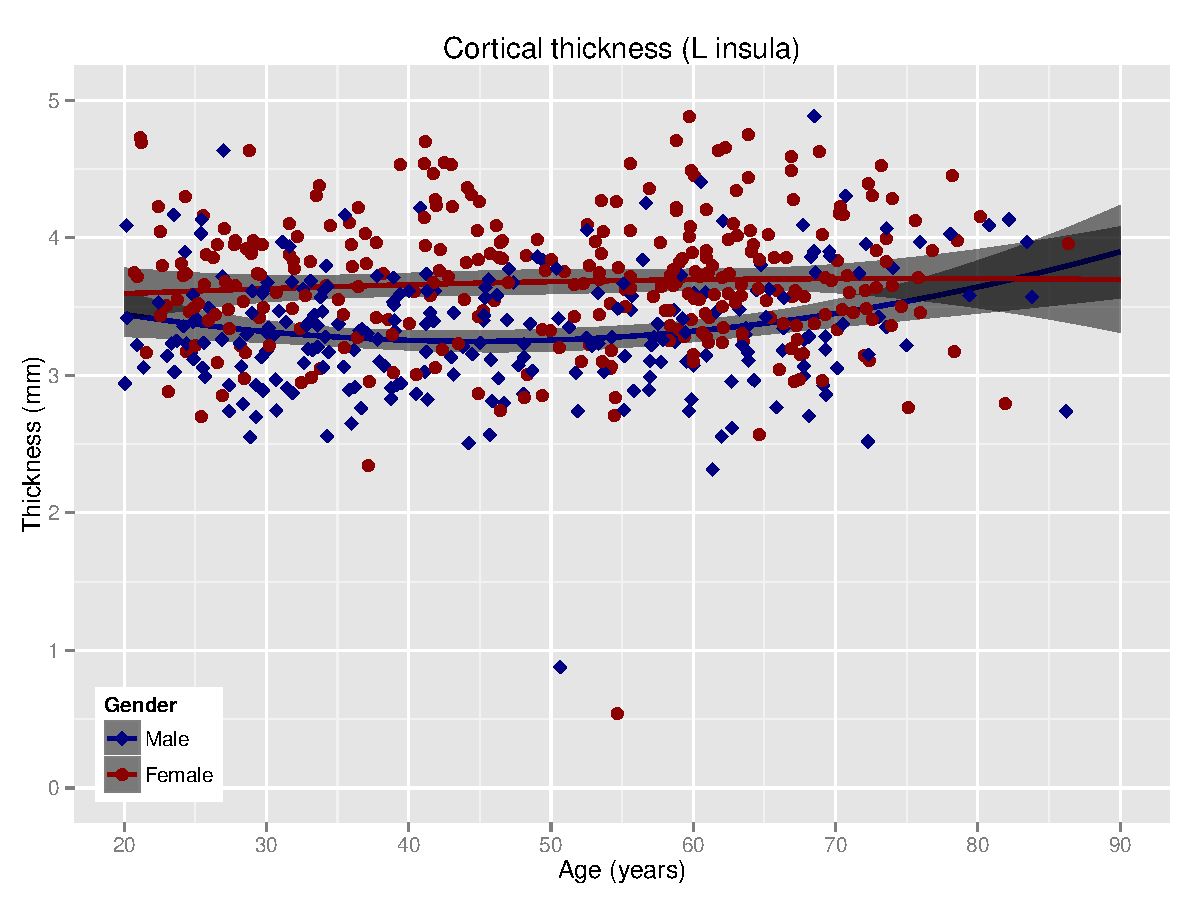
\includegraphics[width=51mm]{IXI_results/yylabel5_results.pdf} &
%  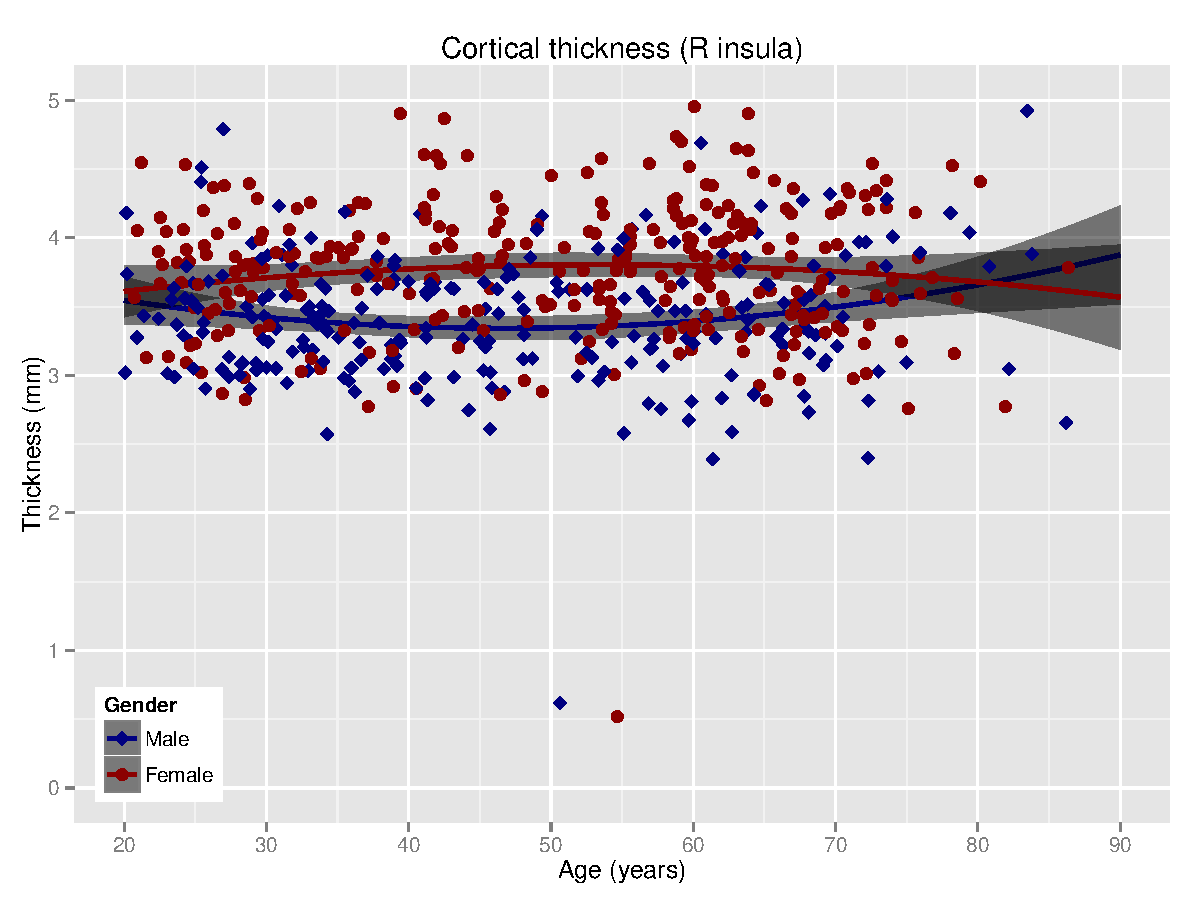
\includegraphics[width=51mm]{IXI_results/yylabel6_results.pdf} &
%  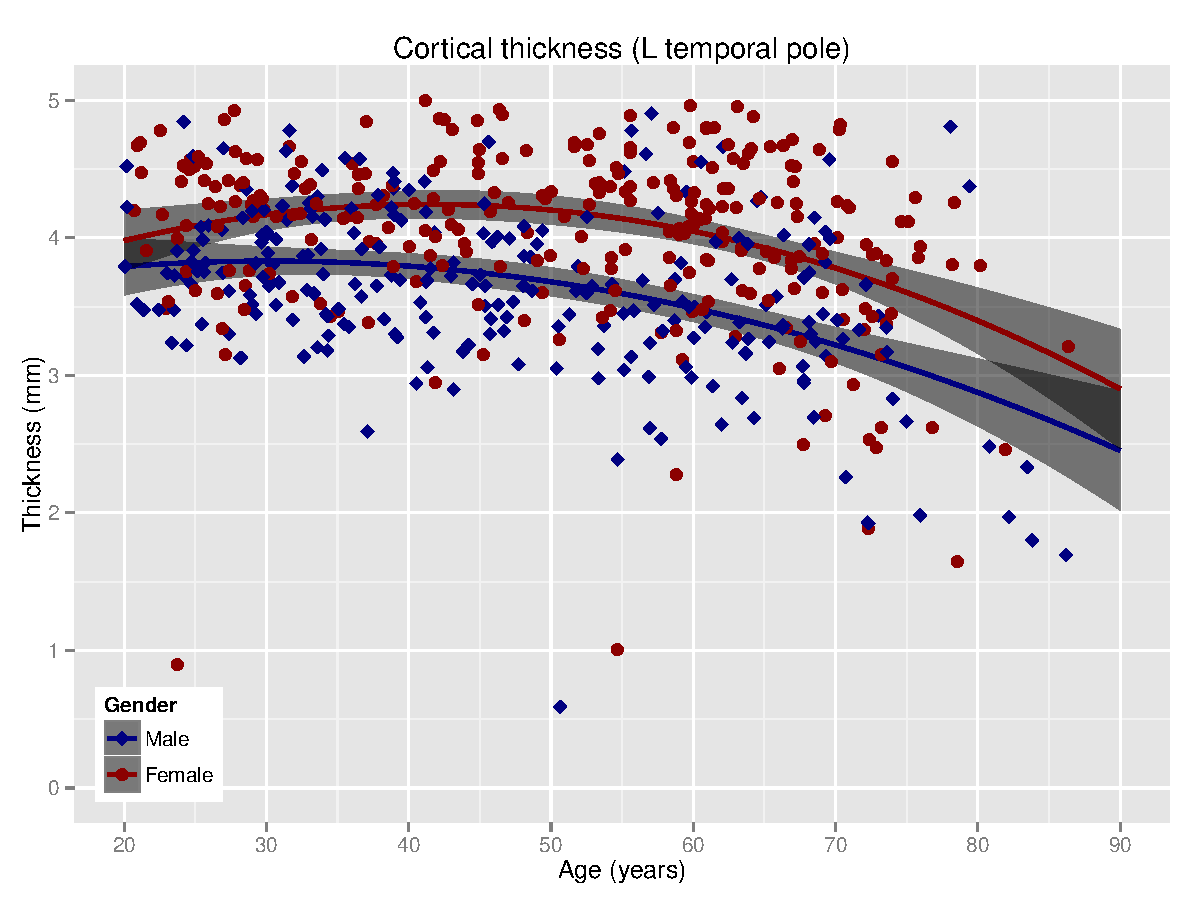
\includegraphics[width=51mm]{IXI_results/yylabel7_results.pdf} &
%  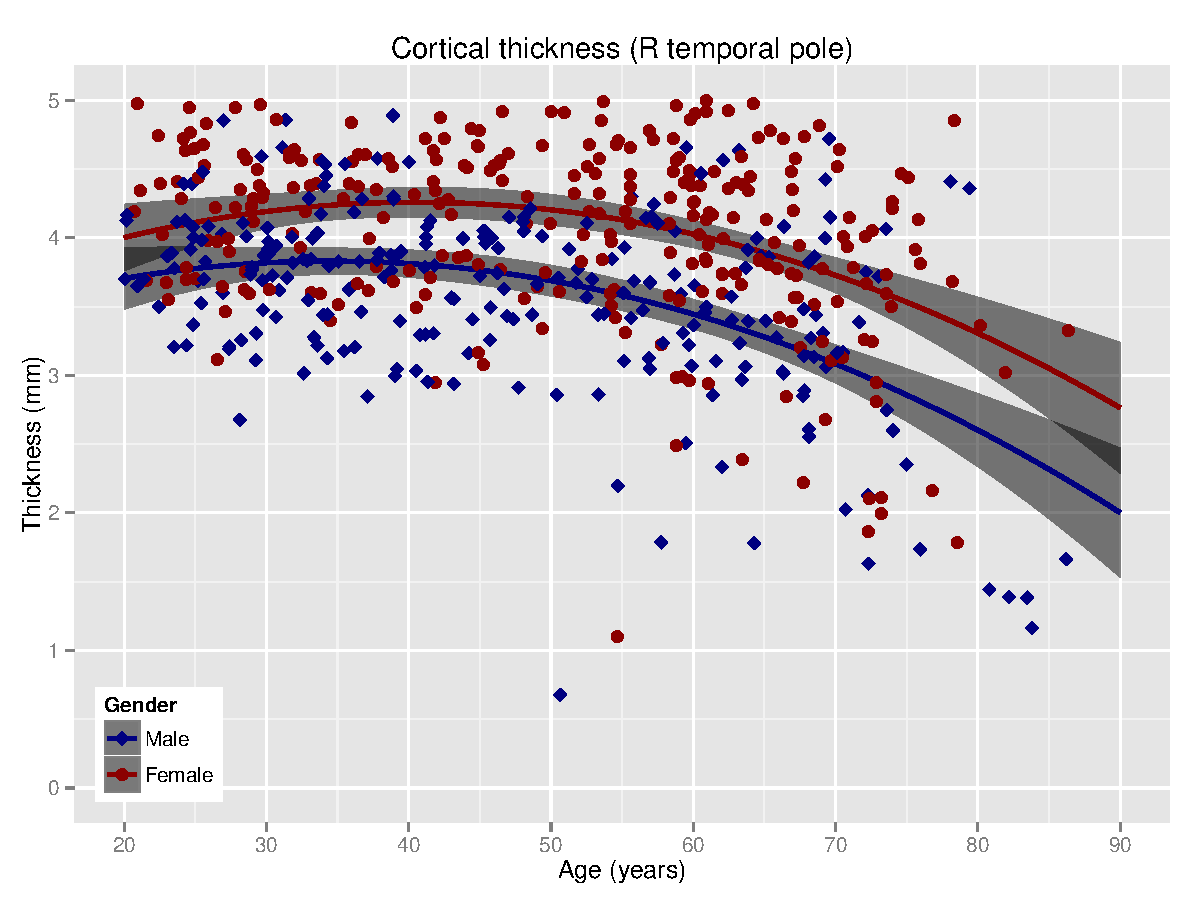
\includegraphics[width=51mm]{IXI_results/yylabel8_results.pdf} \\
%  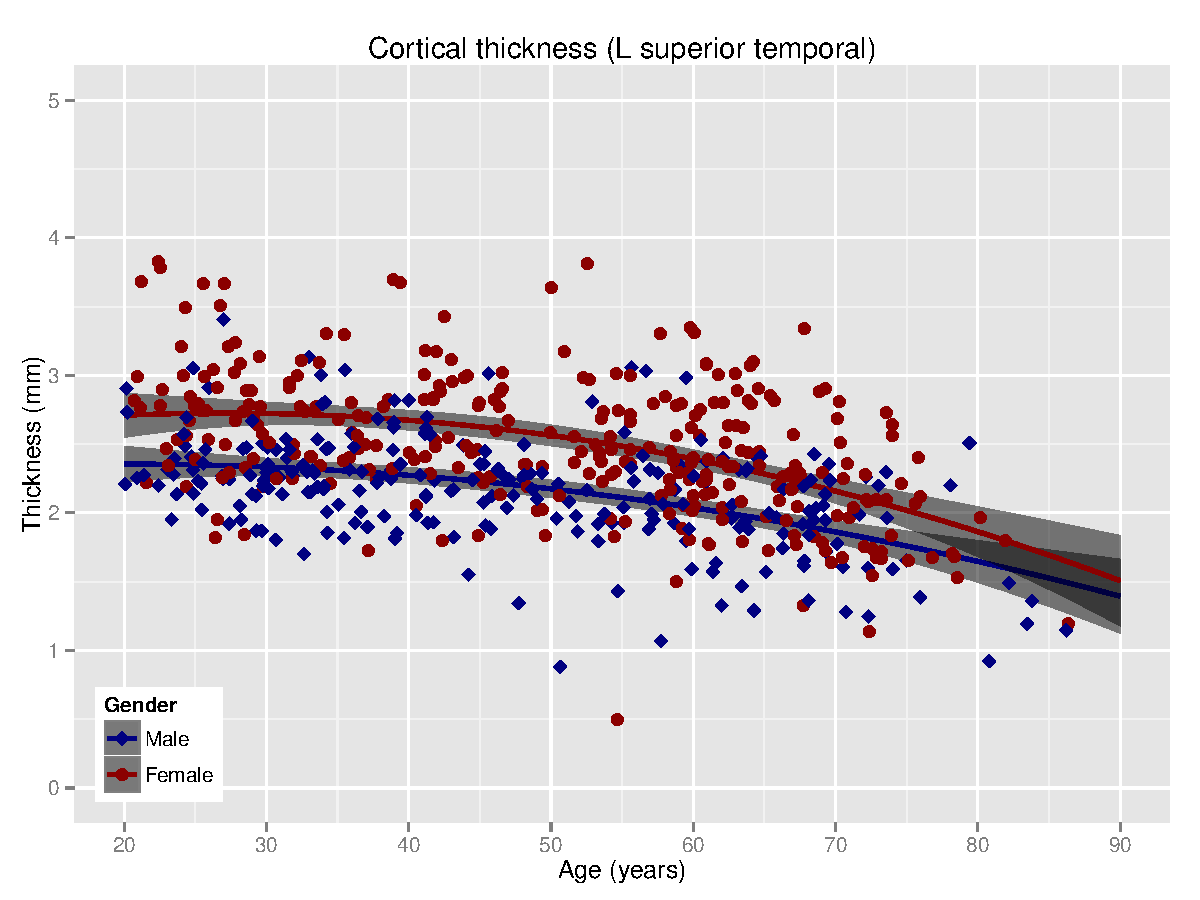
\includegraphics[width=51mm]{IXI_results/yylabel9_results.pdf} &
%  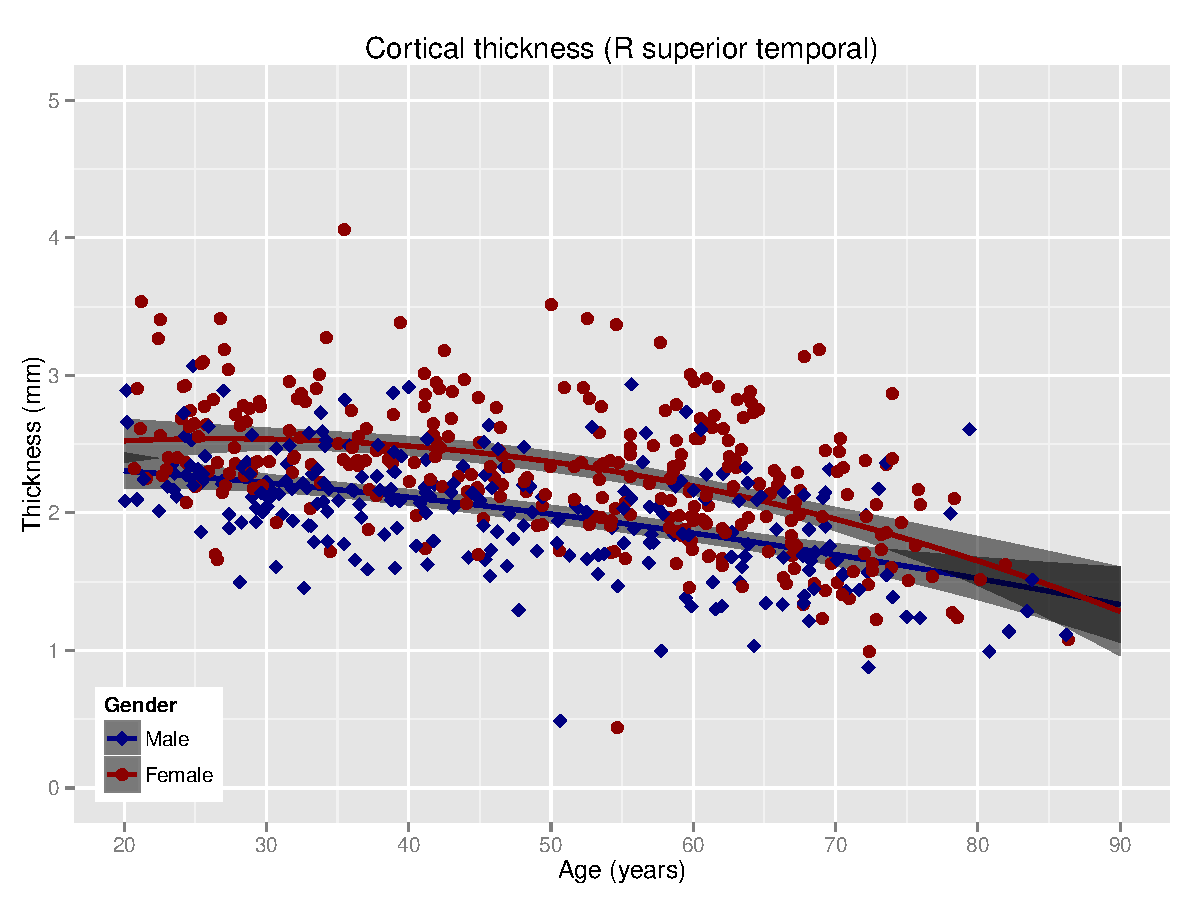
\includegraphics[width=51mm]{IXI_results/yylabel10_results.pdf} &
%  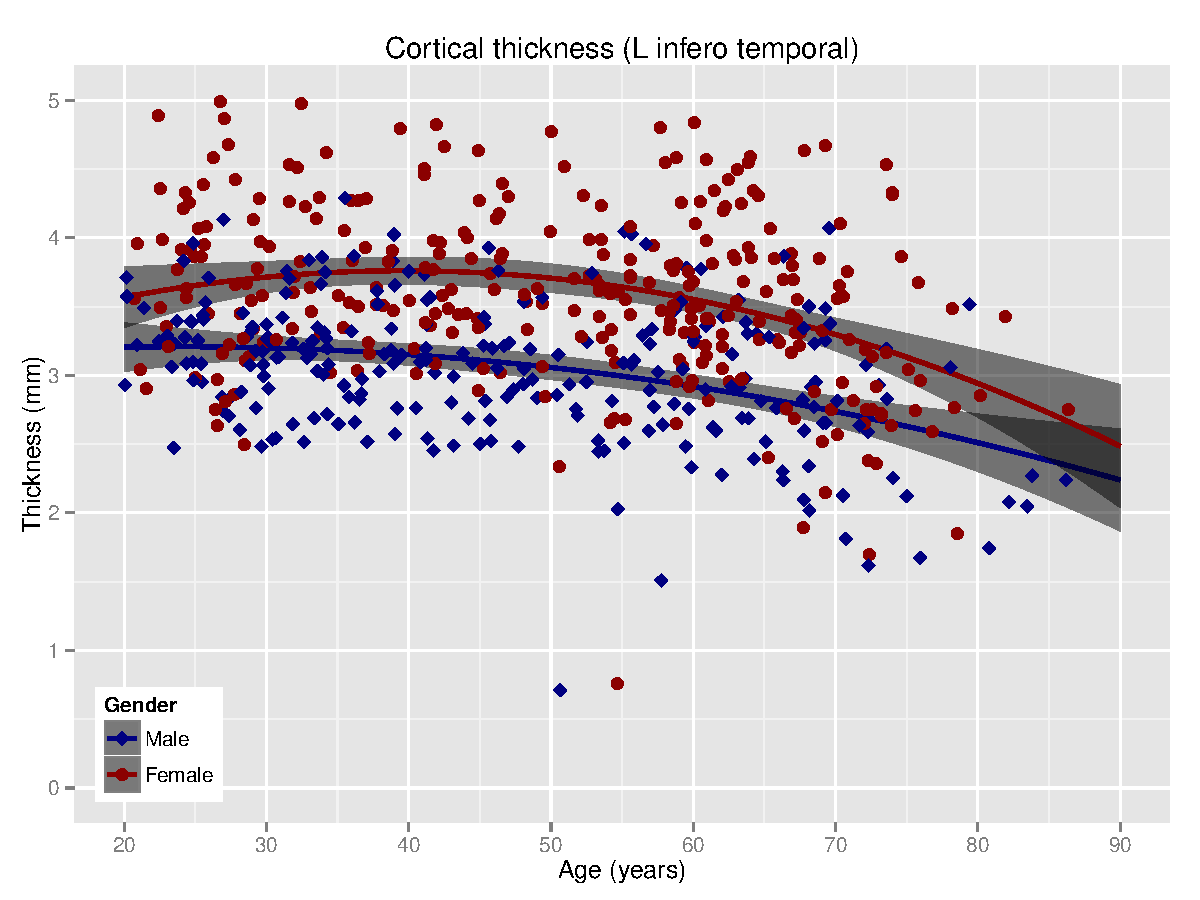
\includegraphics[width=51mm]{IXI_results/yylabel11_results.pdf} &
%  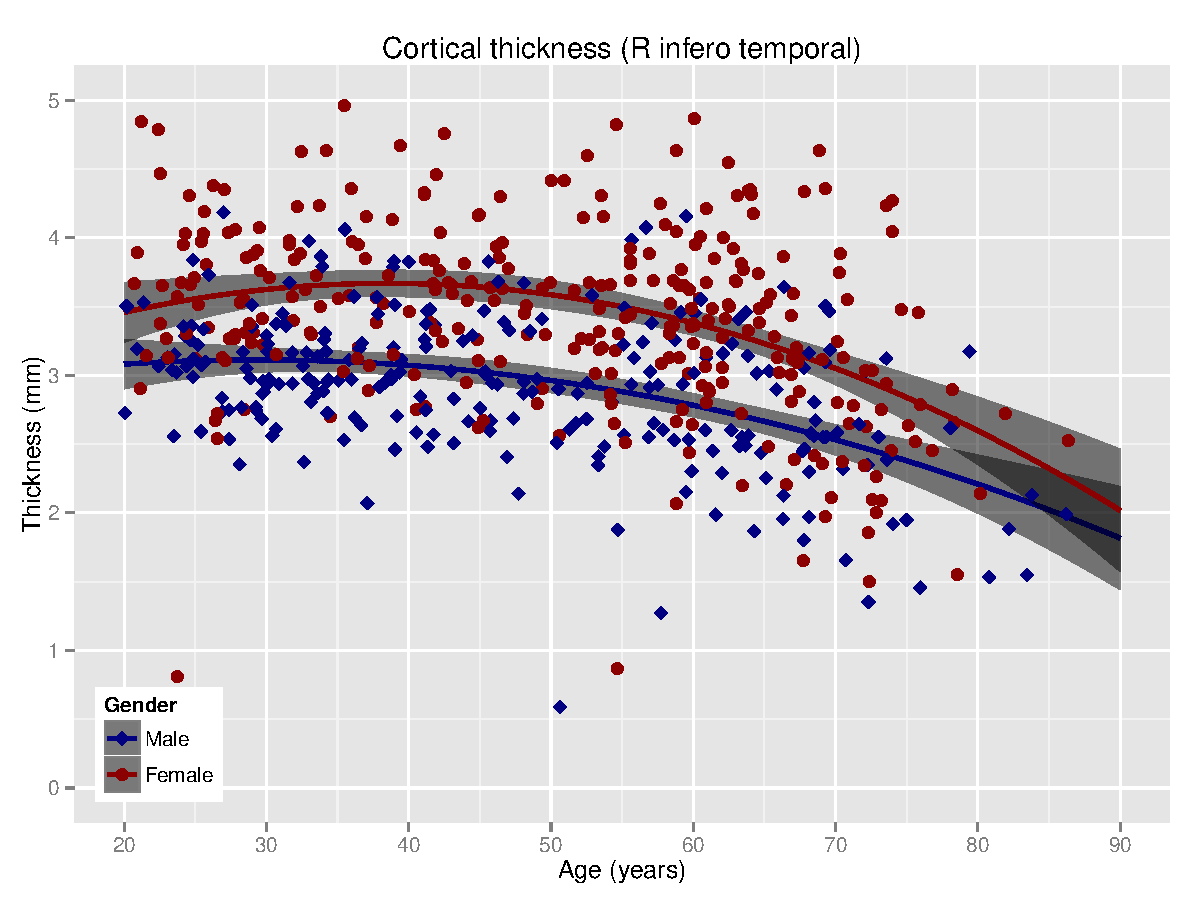
\includegraphics[width=51mm]{IXI_results/yylabel12_results.pdf} \\
%  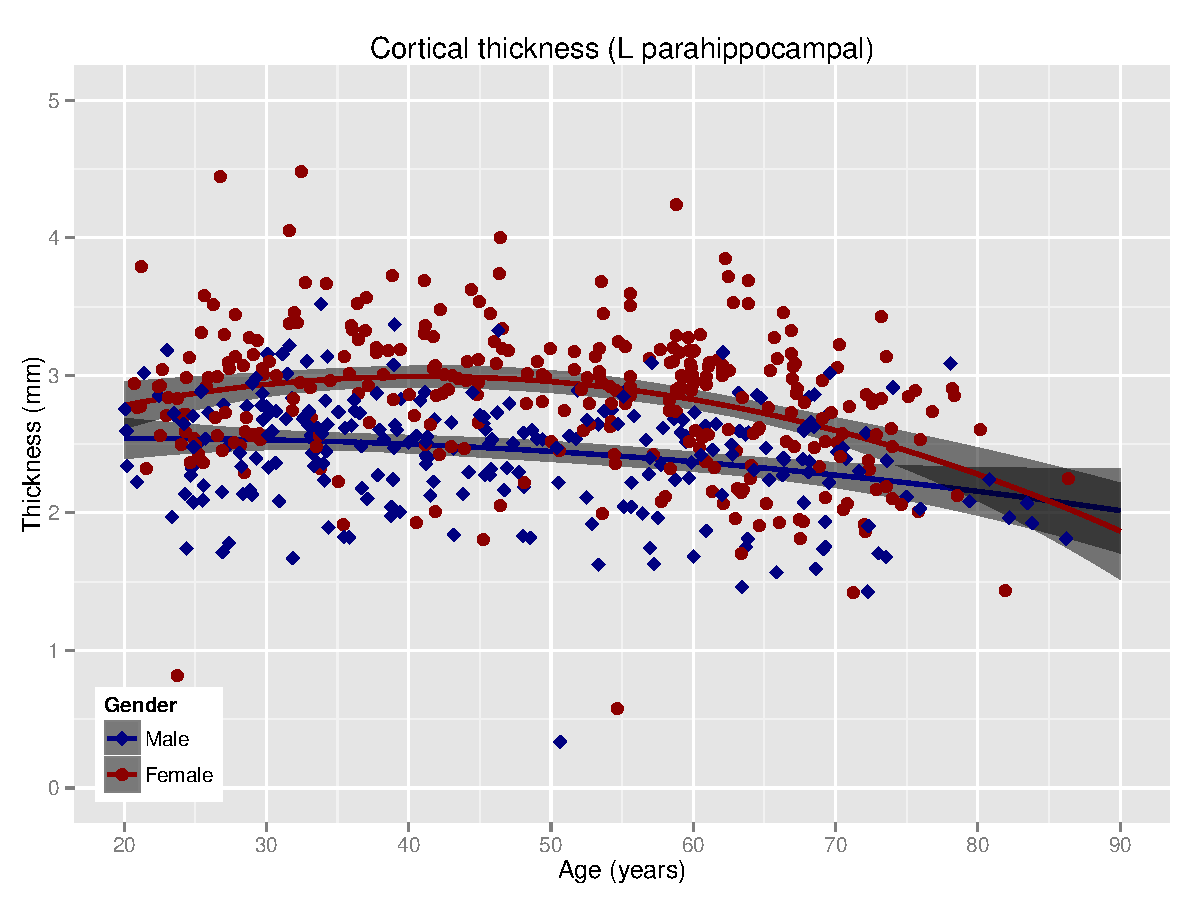
\includegraphics[width=51mm]{IXI_results/yylabel13_results.pdf} &
%  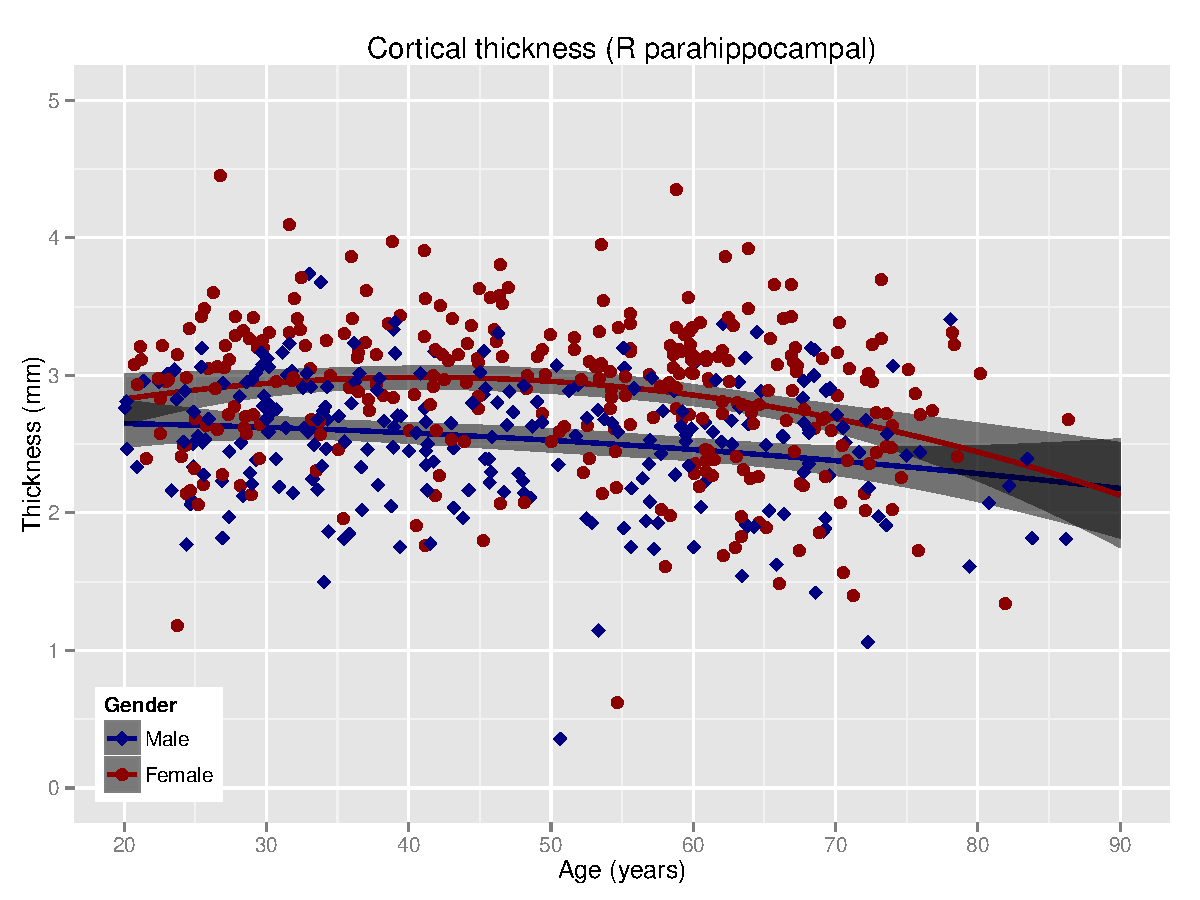
\includegraphics[width=51mm]{IXI_results/yylabel14_results.pdf} &
%  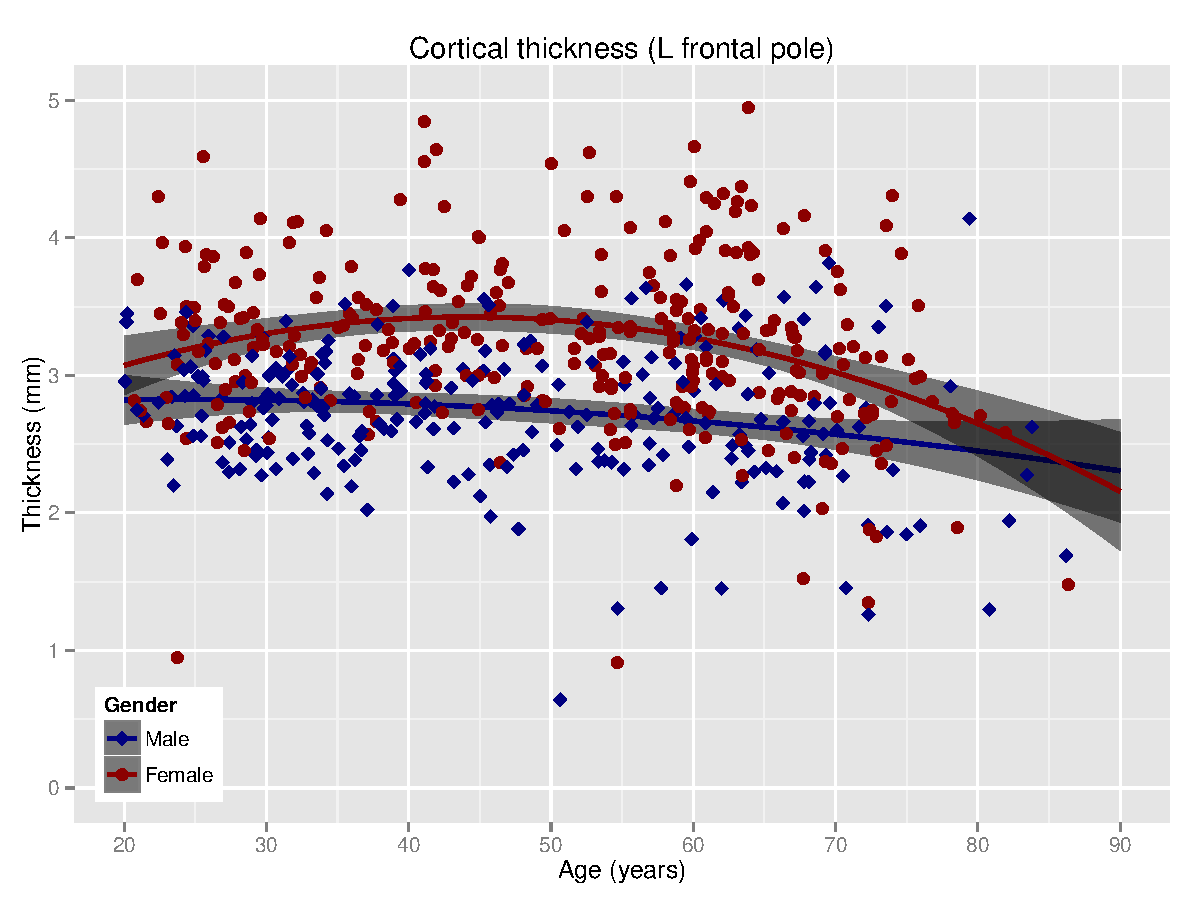
\includegraphics[width=51mm]{IXI_results/yylabel15_results.pdf} &
%  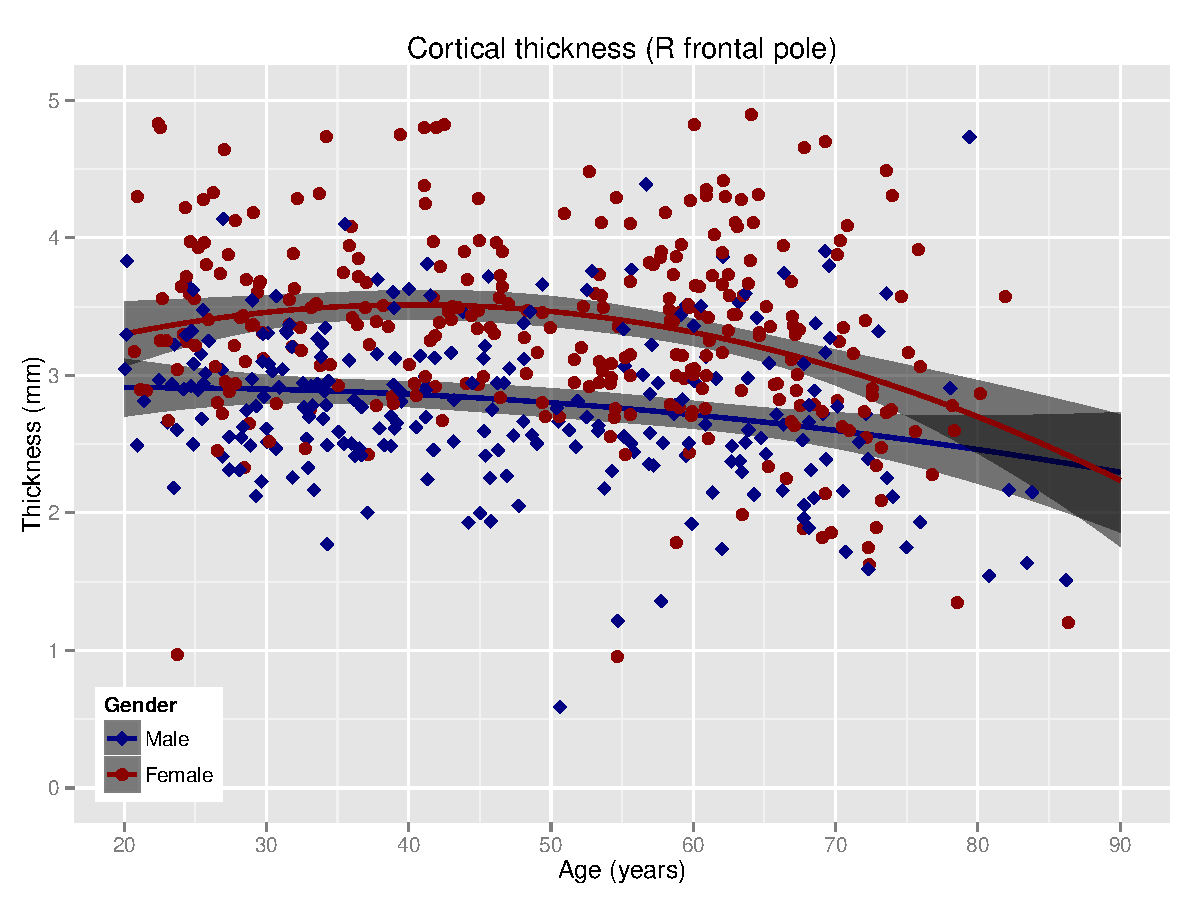
\includegraphics[width=51mm]{IXI_results/yylabel16_results.pdf} \\
%  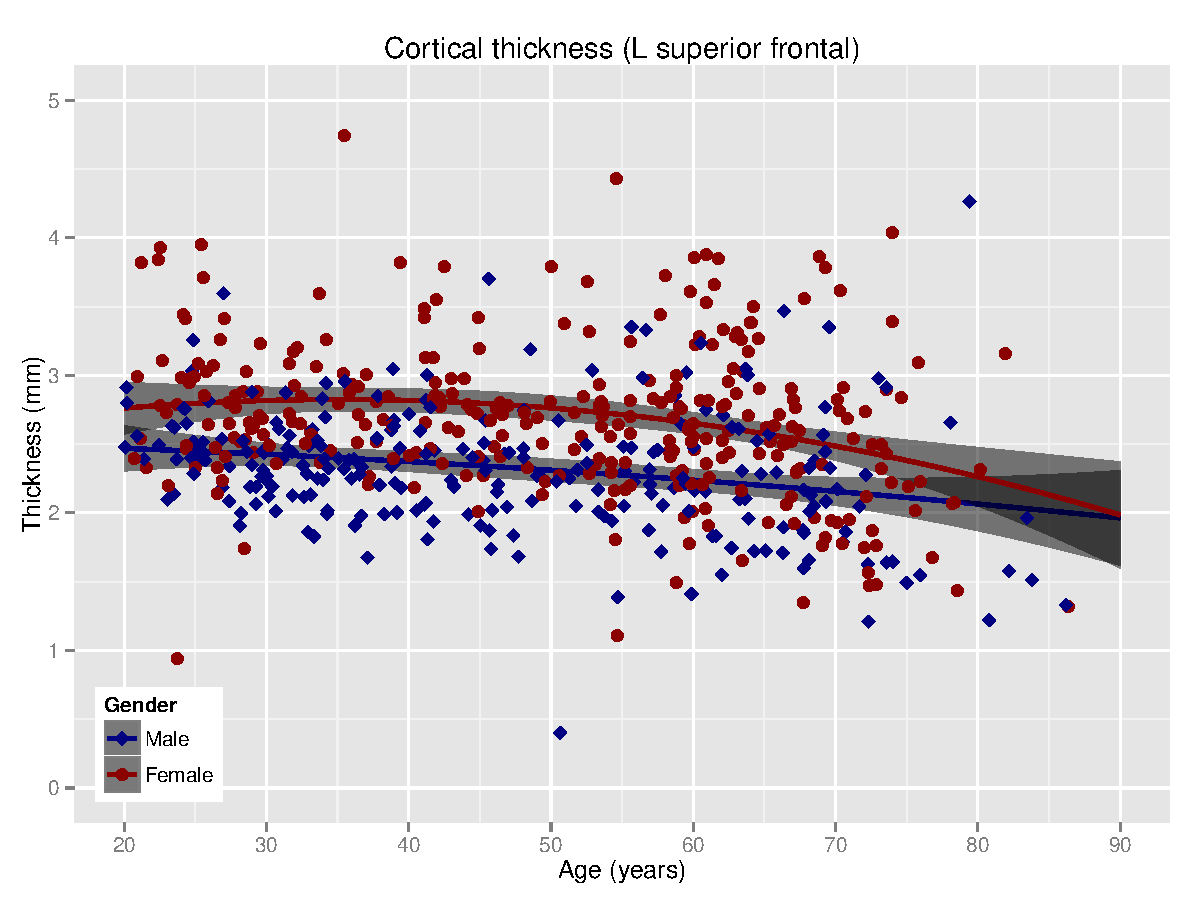
\includegraphics[width=51mm]{IXI_results/yylabel17_results.pdf} &
%  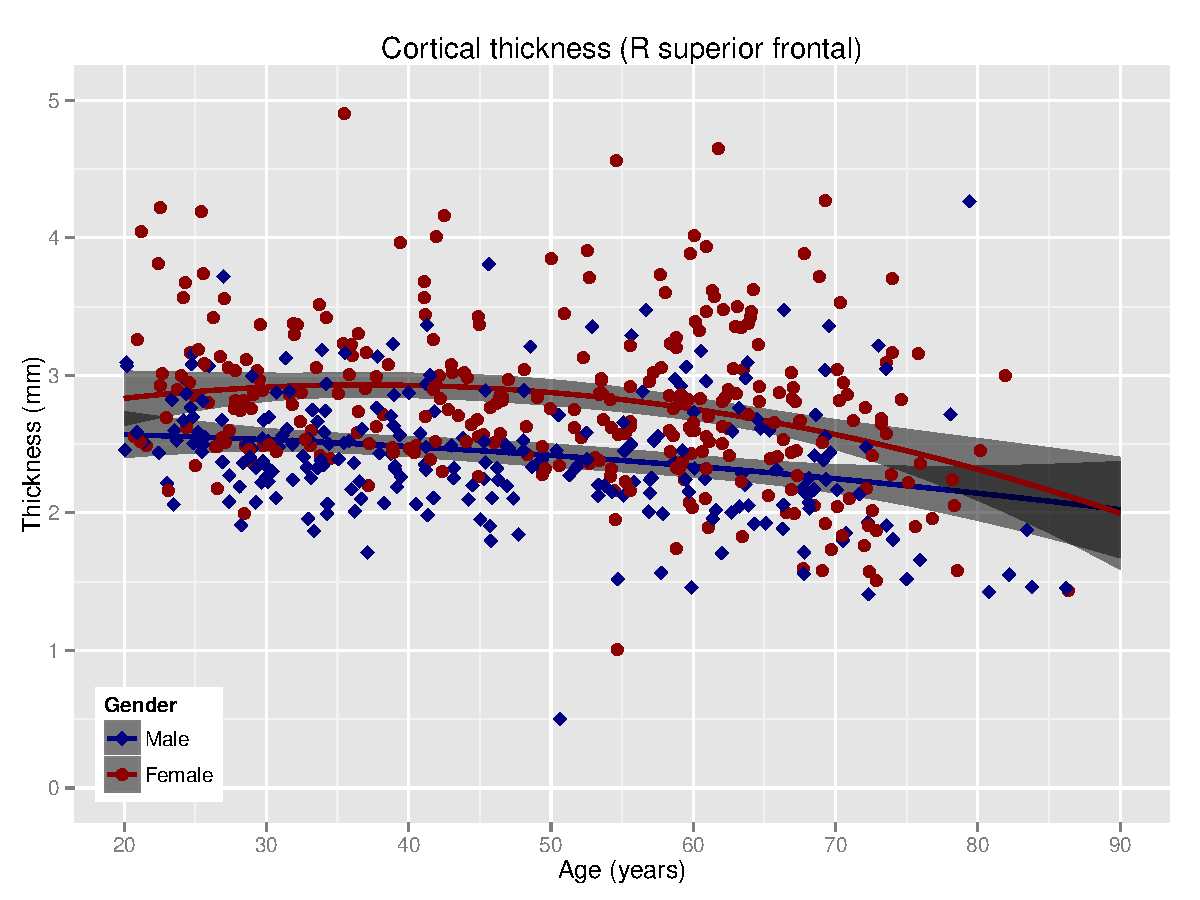
\includegraphics[width=51mm]{IXI_results/yylabel18_results.pdf} &
%  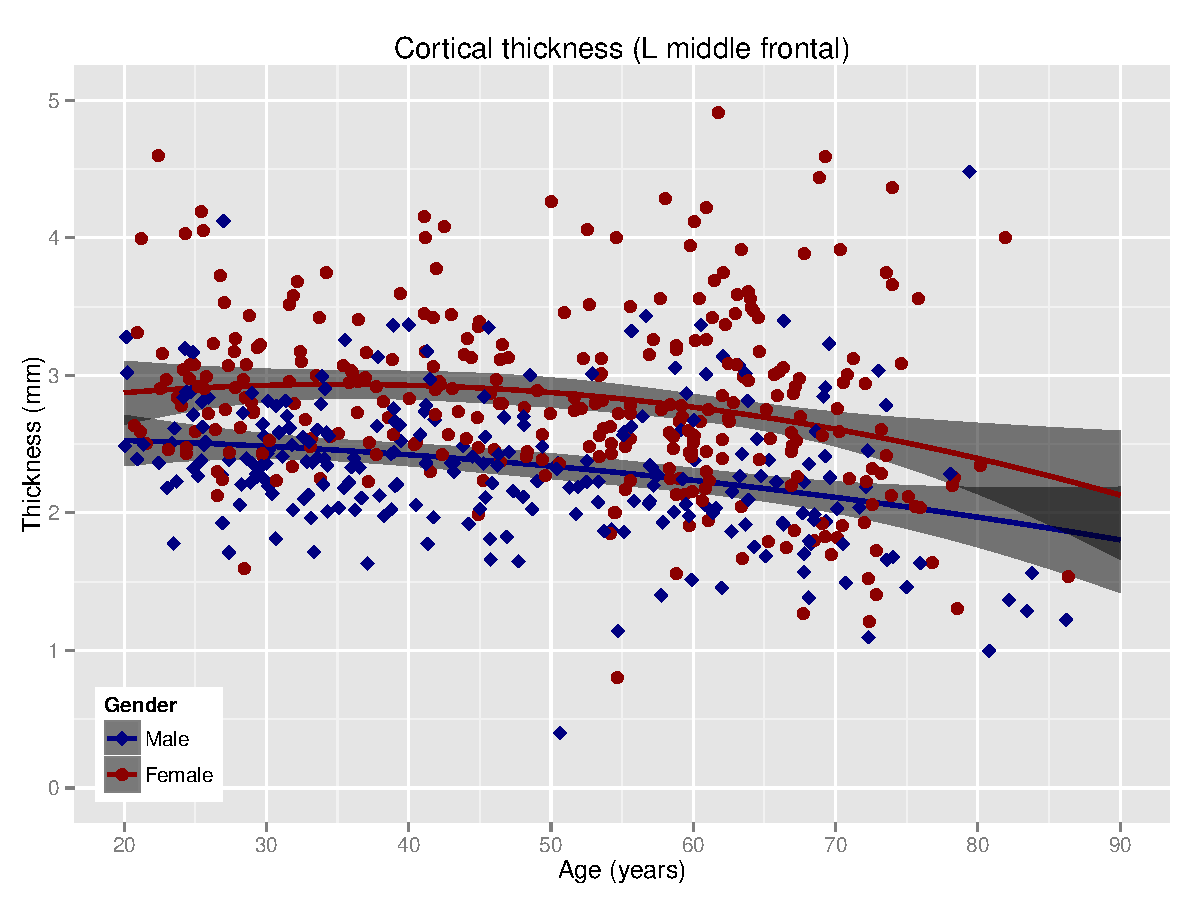
\includegraphics[width=51mm]{IXI_results/yylabel19_results.pdf} &
%  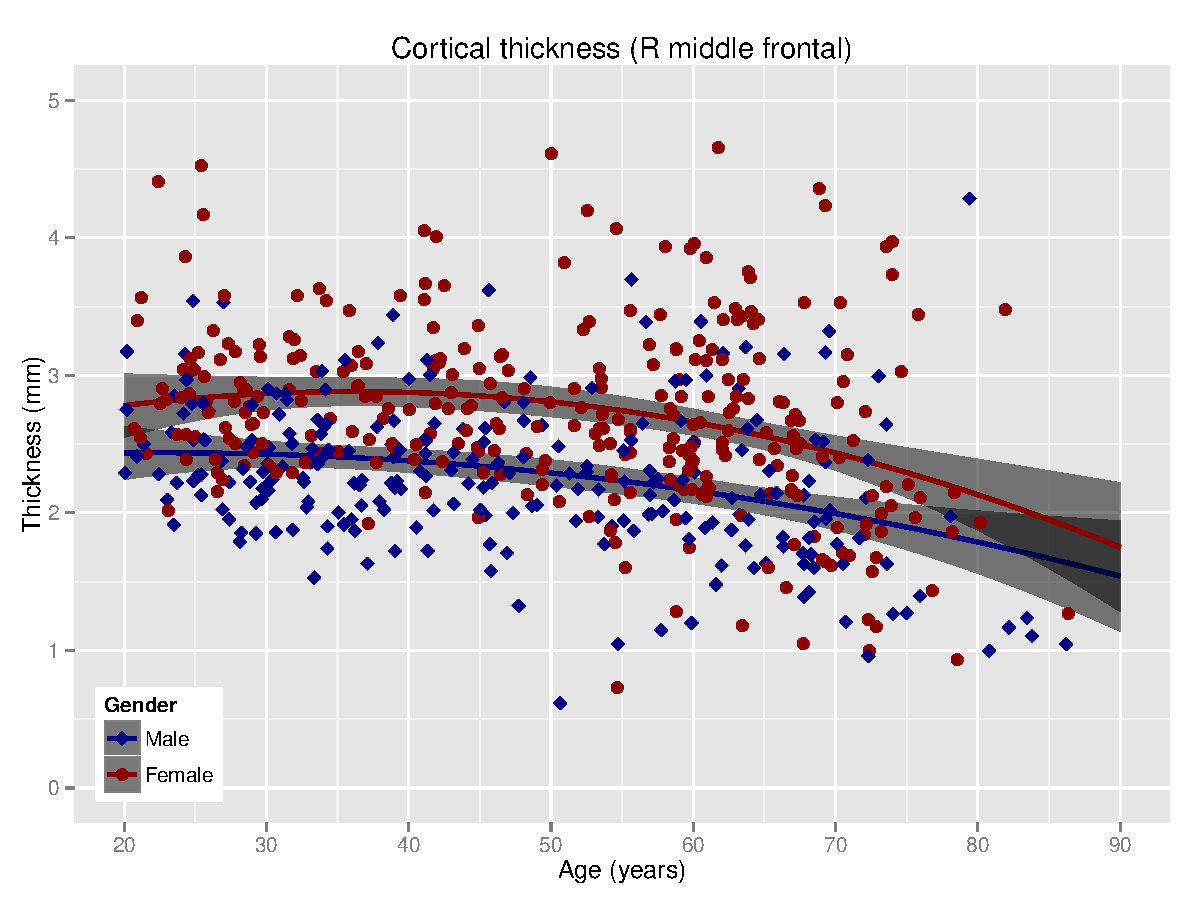
\includegraphics[width=51mm]{IXI_results/yylabel20_results.pdf} \\
%  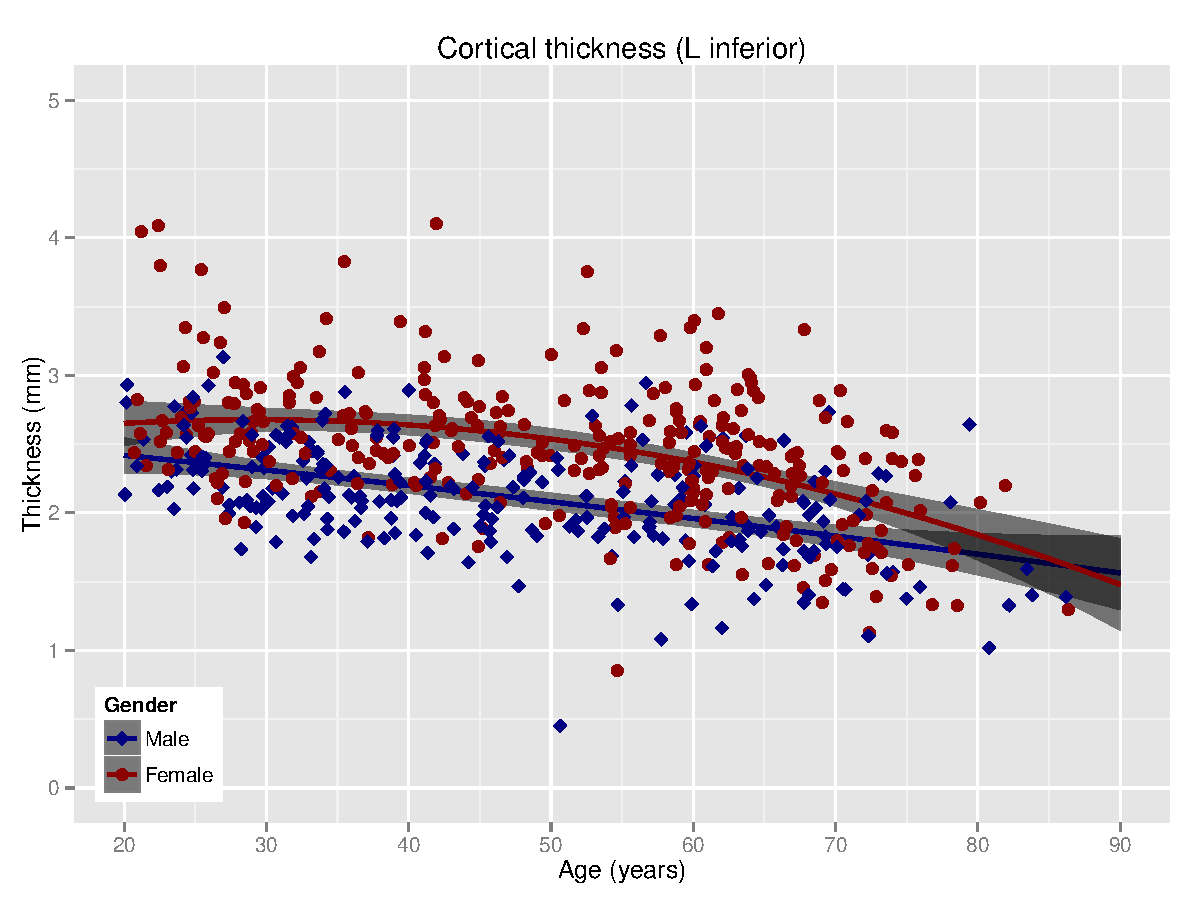
\includegraphics[width=51mm]{IXI_results/yylabel21_results.pdf} &
%  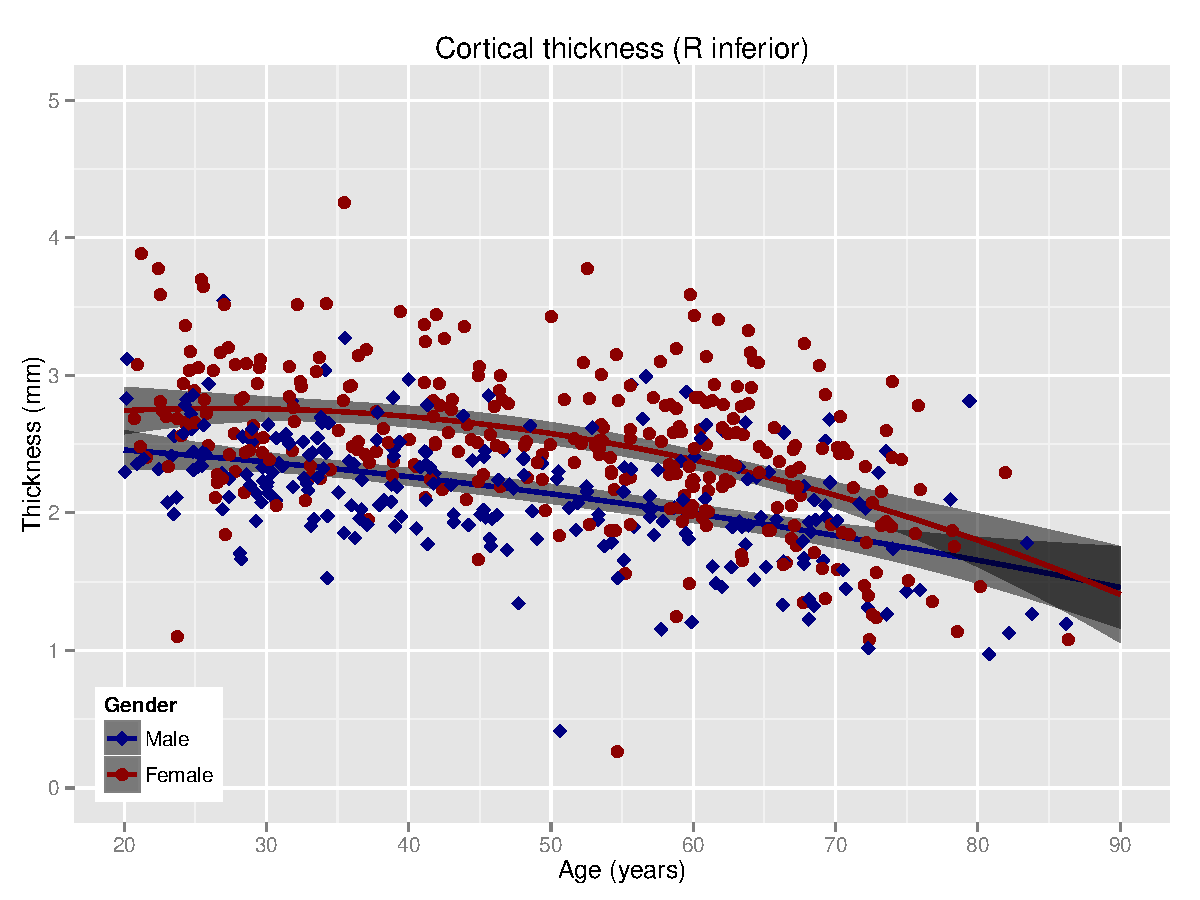
\includegraphics[width=51mm]{IXI_results/yylabel22_results.pdf} &
%  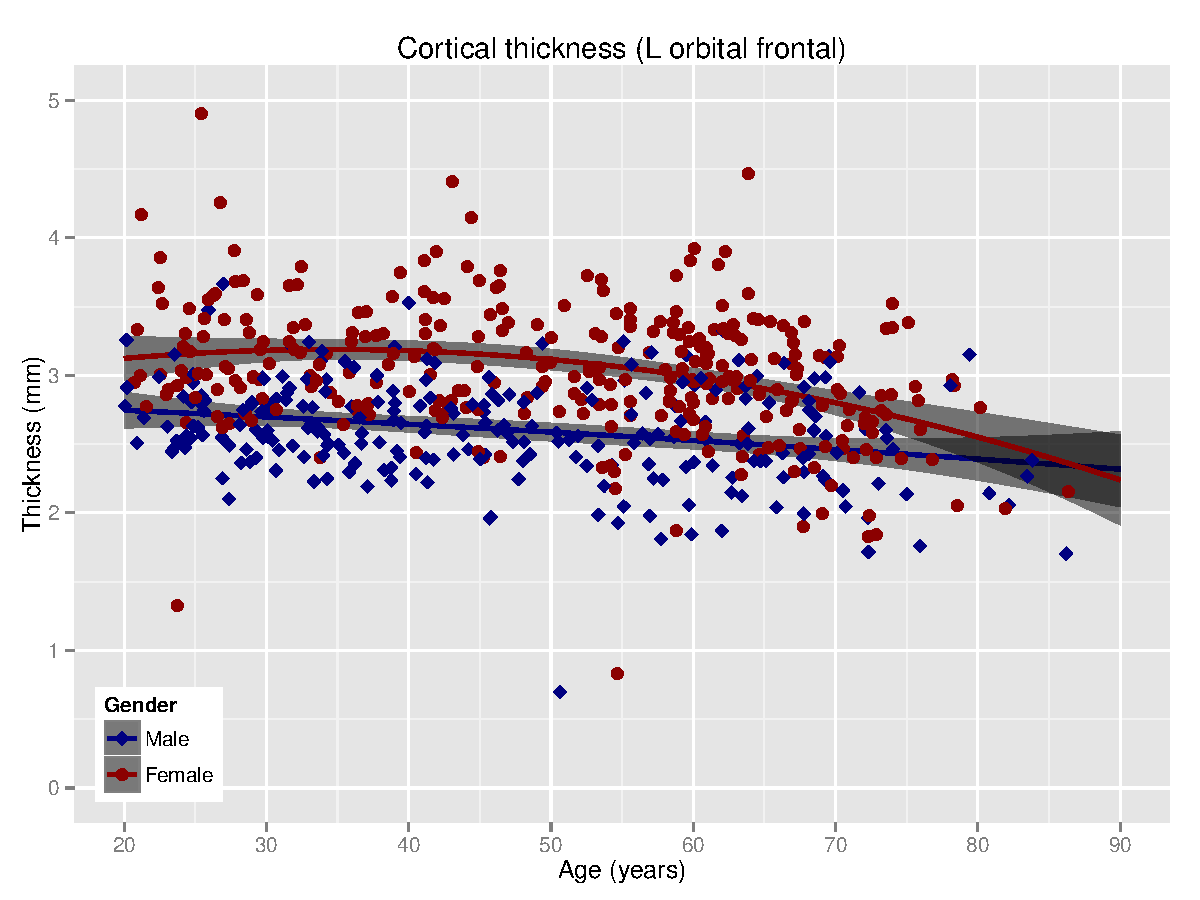
\includegraphics[width=51mm]{IXI_results/yylabel23_results.pdf} &
%  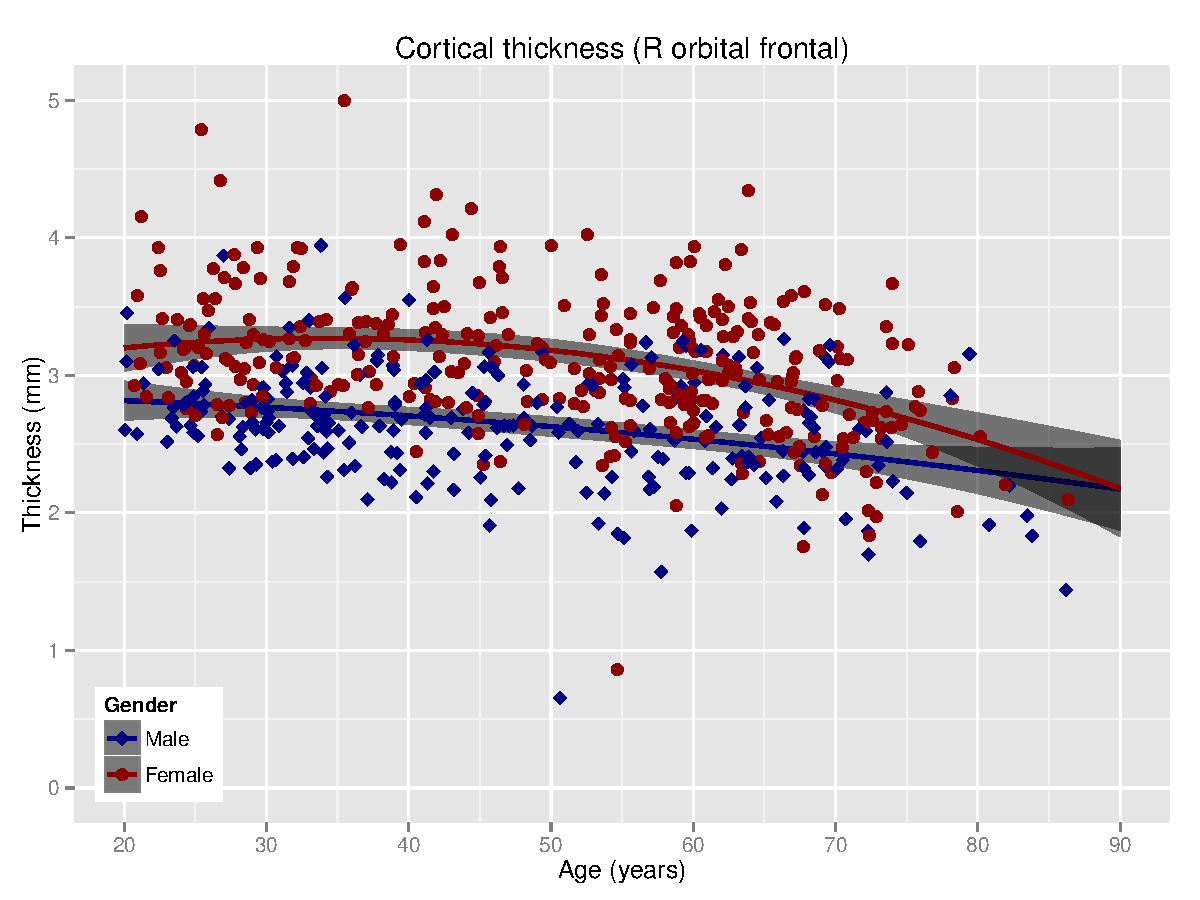
\includegraphics[width=51mm]{IXI_results/yylabel24_results.pdf} \\
%  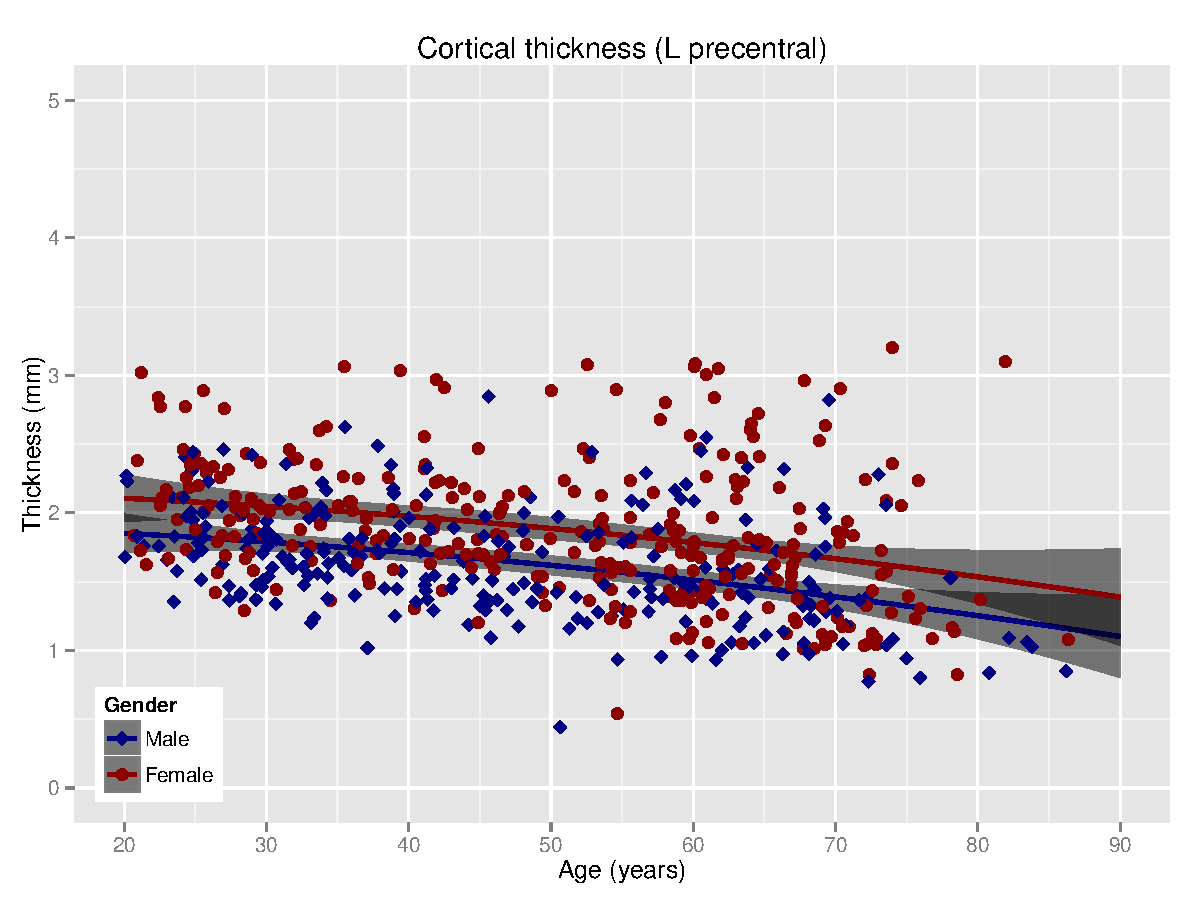
\includegraphics[width=51mm]{IXI_results/yylabel25_results.pdf} &
%  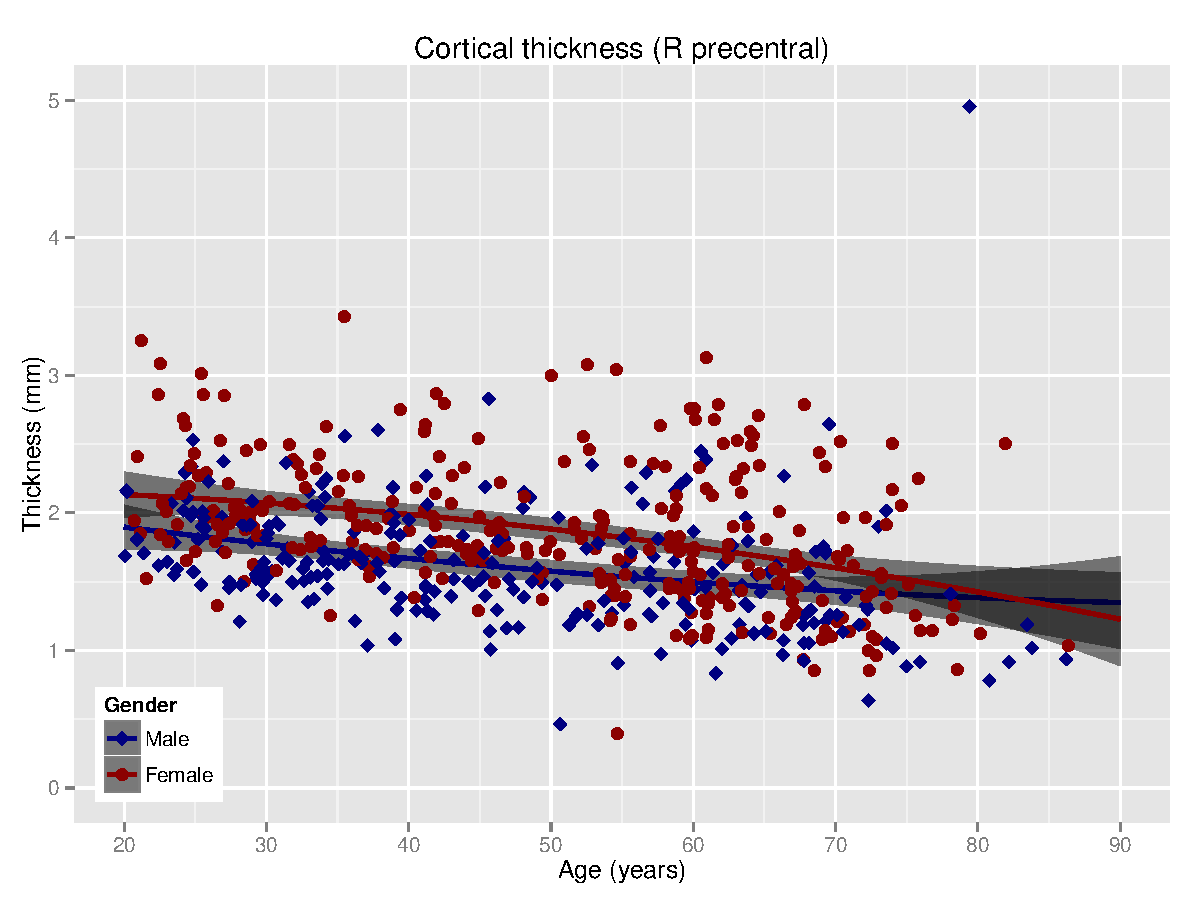
\includegraphics[width=51mm]{IXI_results/yylabel26_results.pdf} &
%  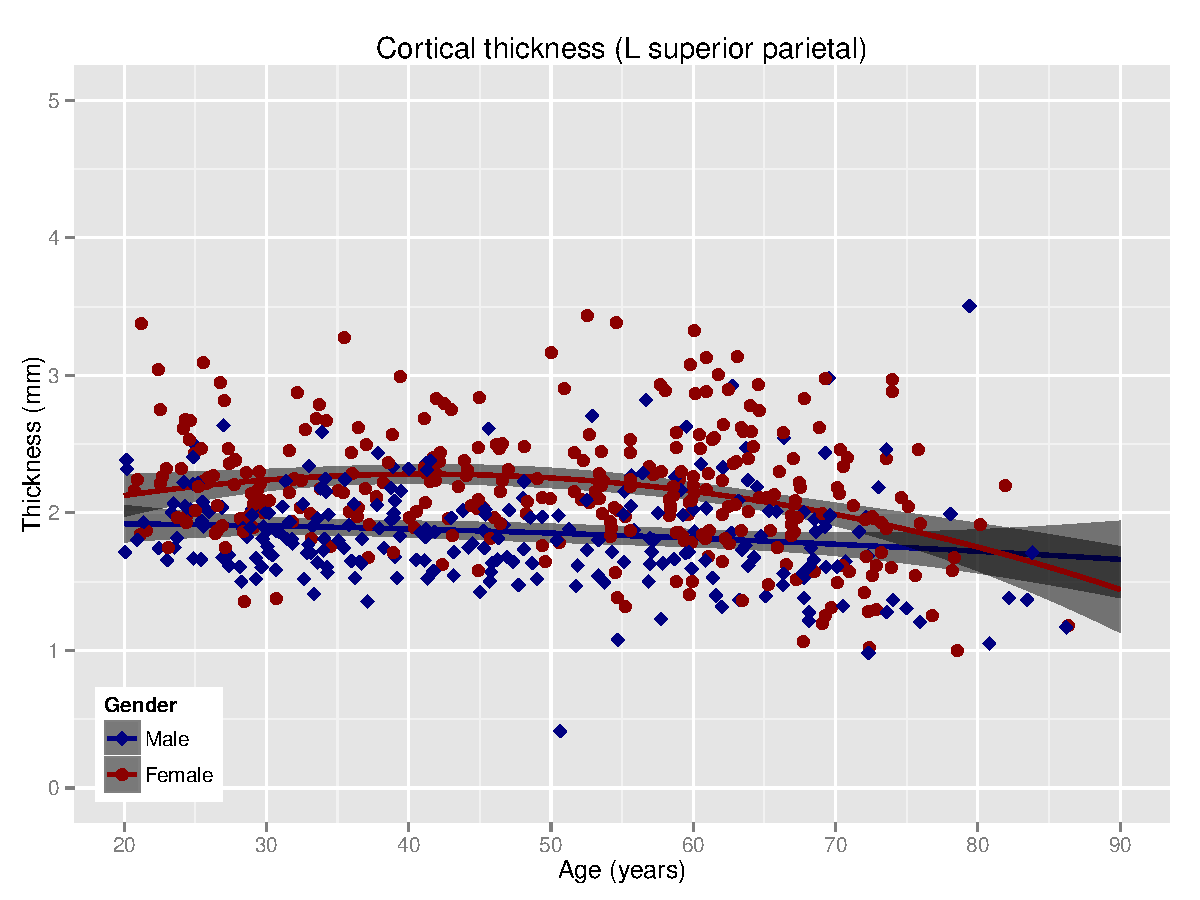
\includegraphics[width=51mm]{IXI_results/yylabel27_results.pdf} &
%  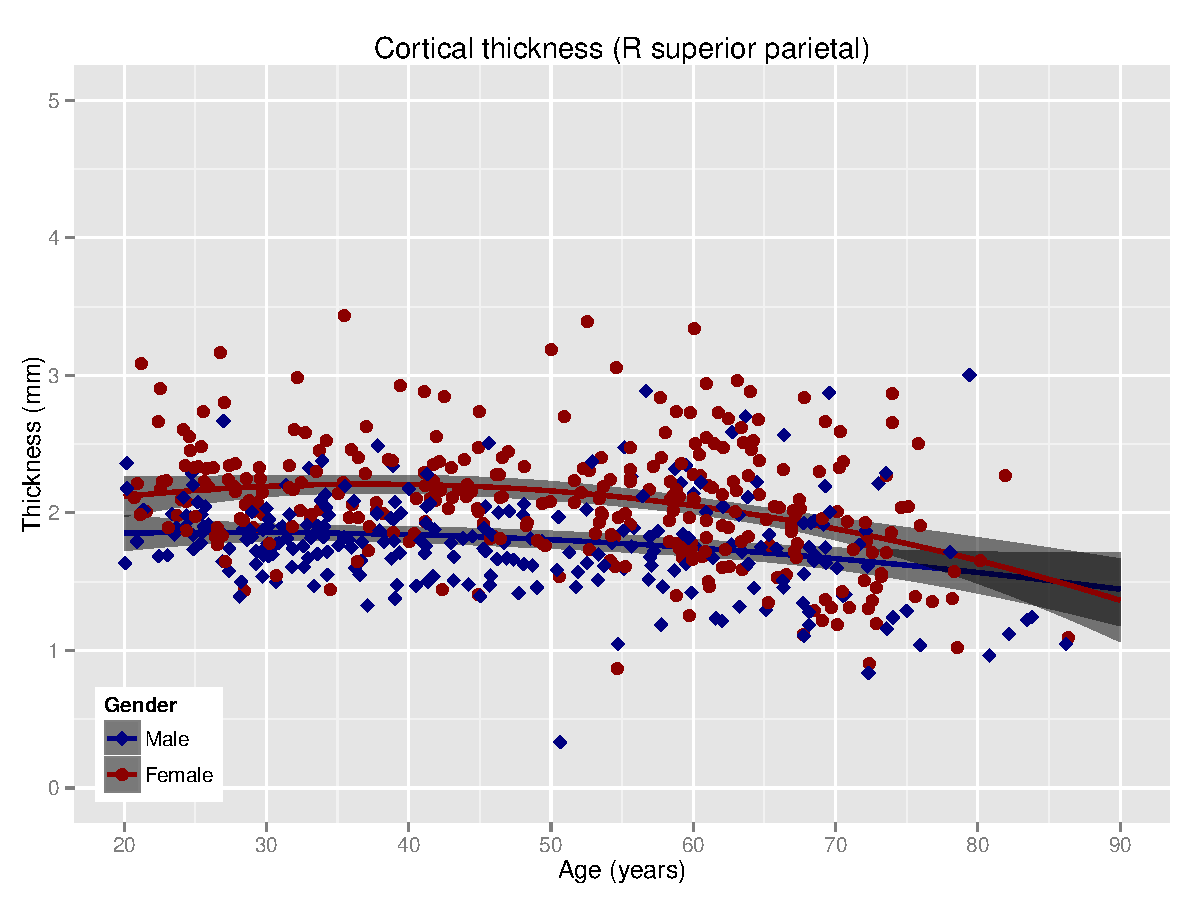
\includegraphics[width=51mm]{IXI_results/yylabel28_results.pdf} \\
%  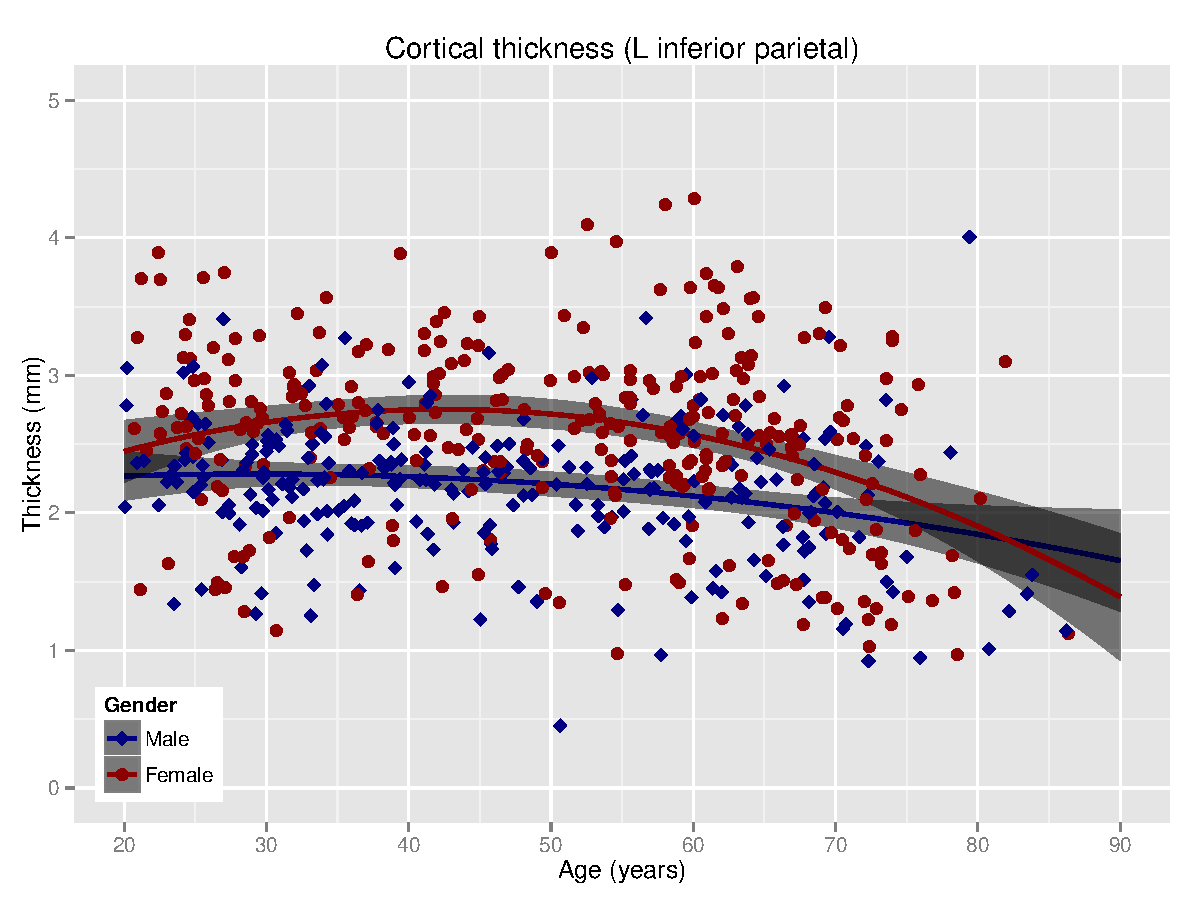
\includegraphics[width=51mm]{IXI_results/yylabel29_results.pdf} &
%  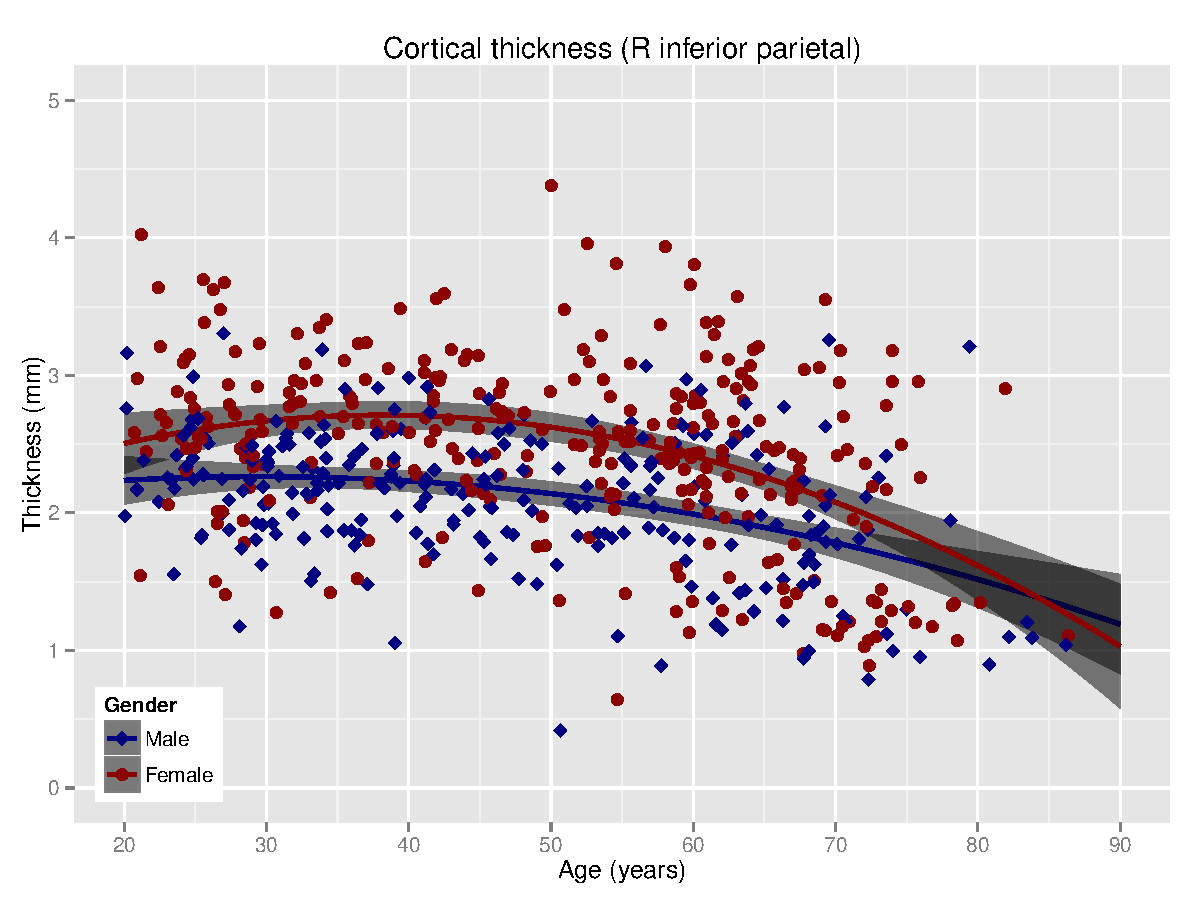
\includegraphics[width=51mm]{IXI_results/yylabel30_results.pdf} &
%  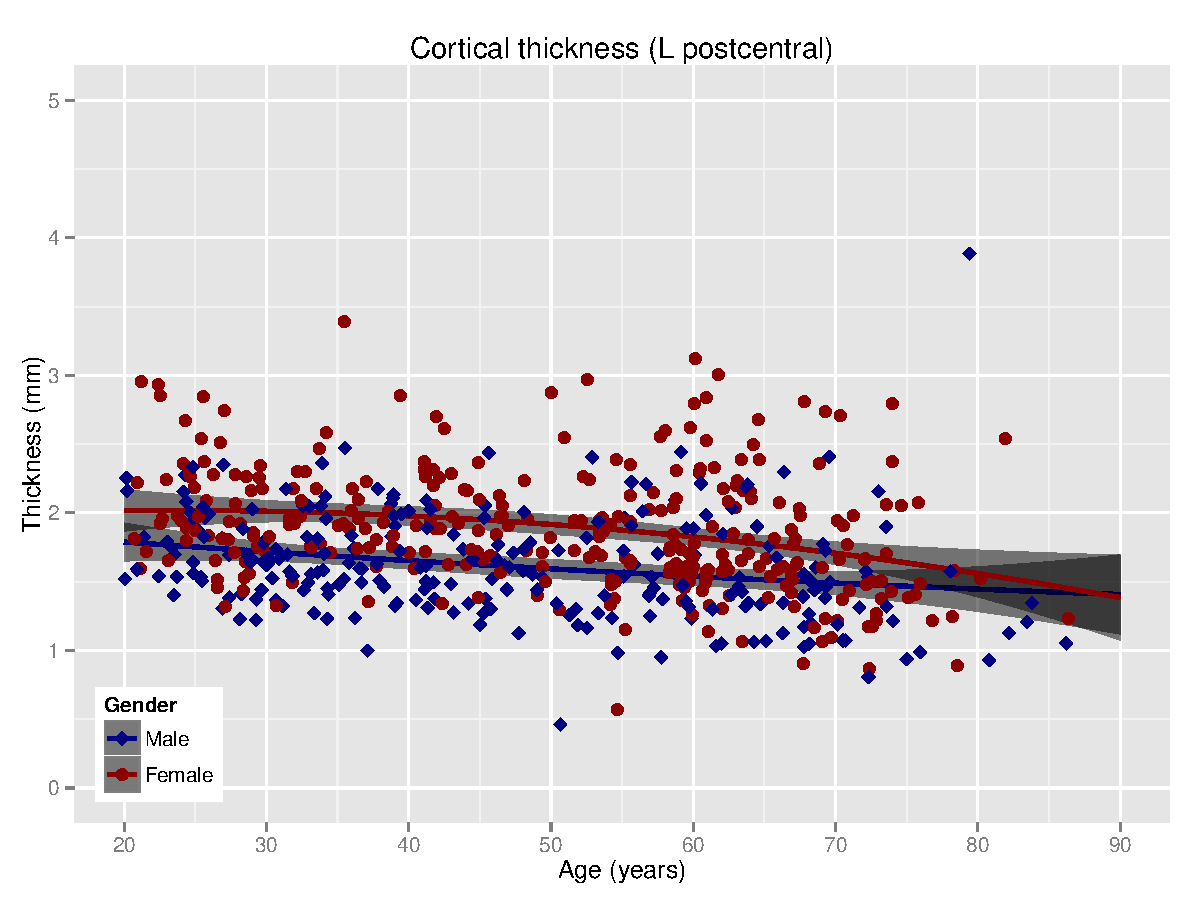
\includegraphics[width=51mm]{IXI_results/yylabel31_results.pdf} &
%  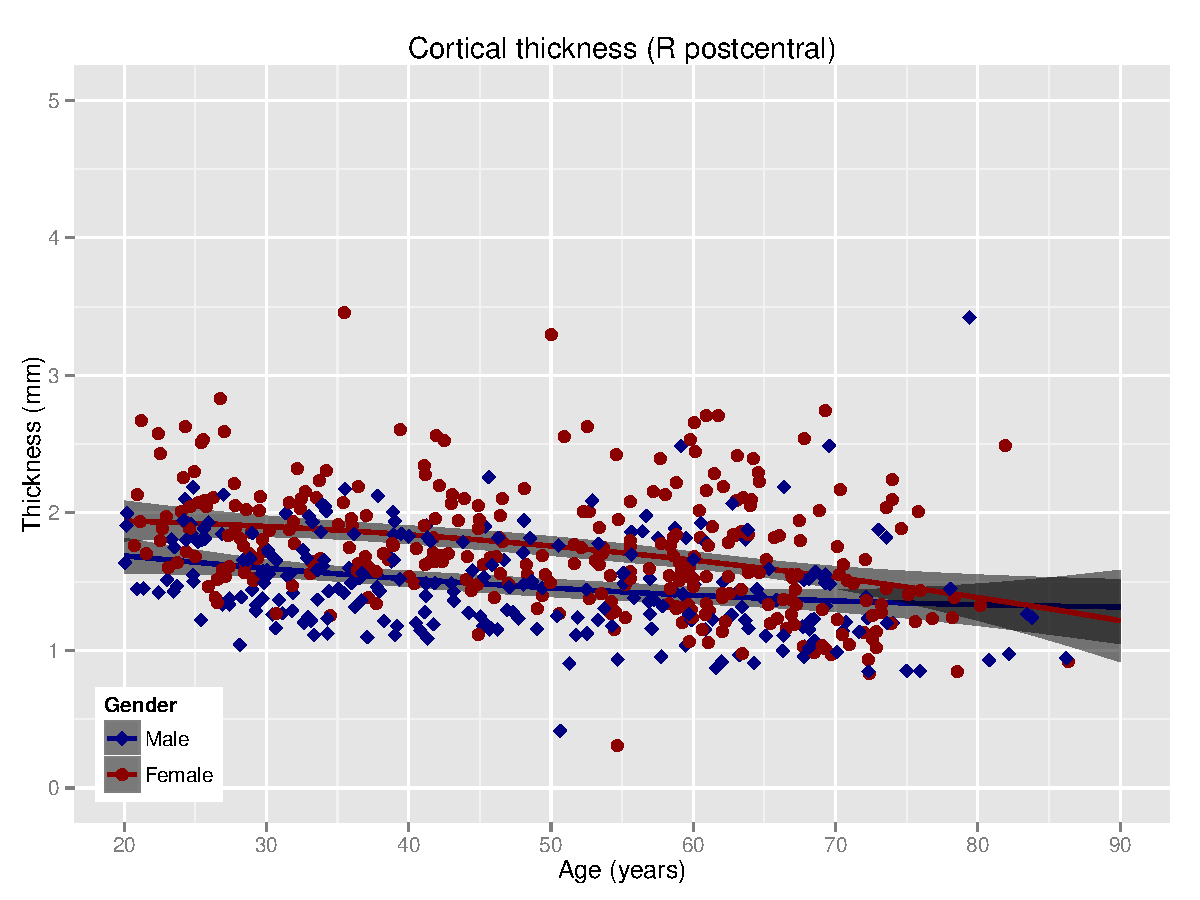
\includegraphics[width=51mm]{IXI_results/yylabel32_results.pdf} 
%  \end{tabular}
%  \caption{Cortical thickness results (age vs. thickness) from the IXI data set where
%  each plot corresponds to one of the 32 cortical labels from the NIREP NA0 data set.  
%  Thickness values have been normalized corresponding to the ratio of the individual 
%  subject volume versus the total template volume.
%  }
%  \label{fig:nirep}
%\end{figure}


\begin{figure}
  \centering
  \begin{tabular}{ccc}
  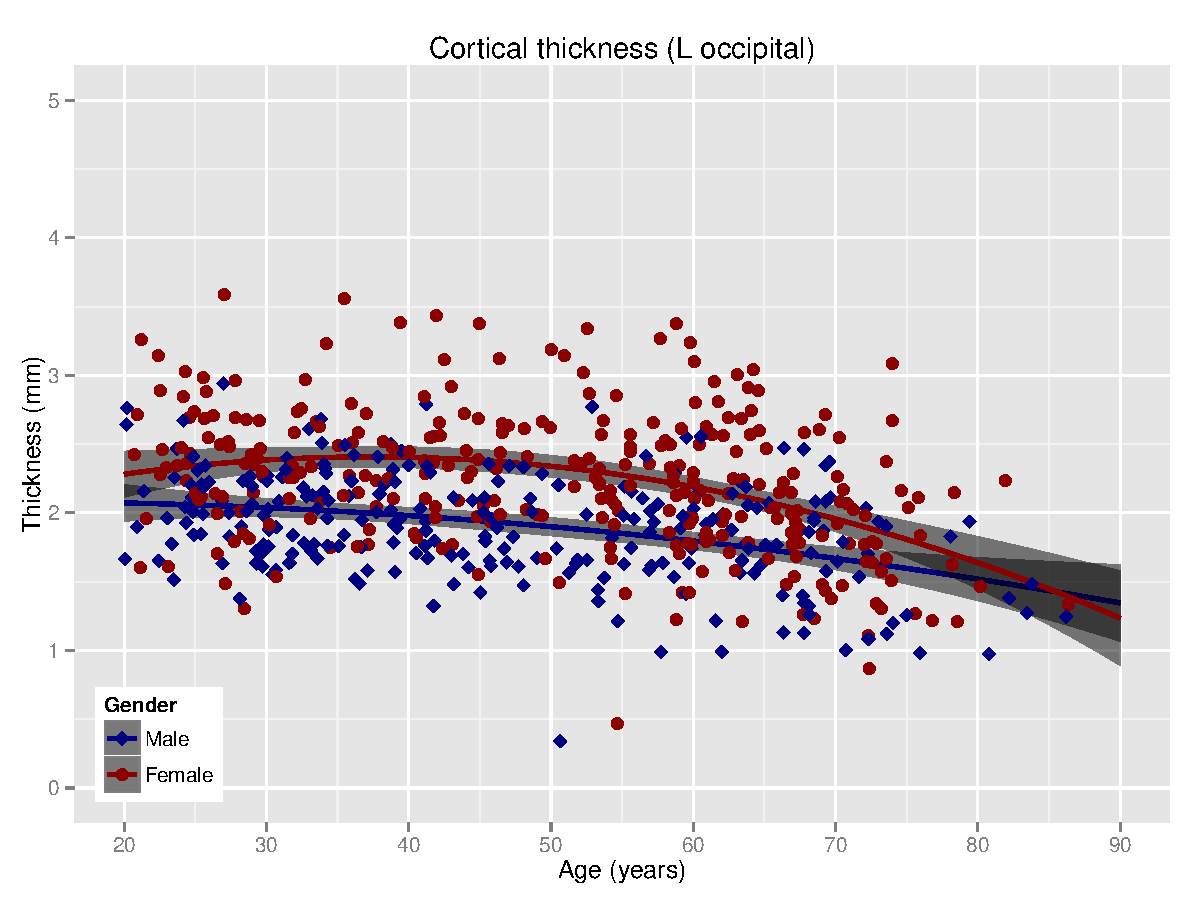
\includegraphics[width=51mm]{IXI_results/yylabel1_results.pdf} &
  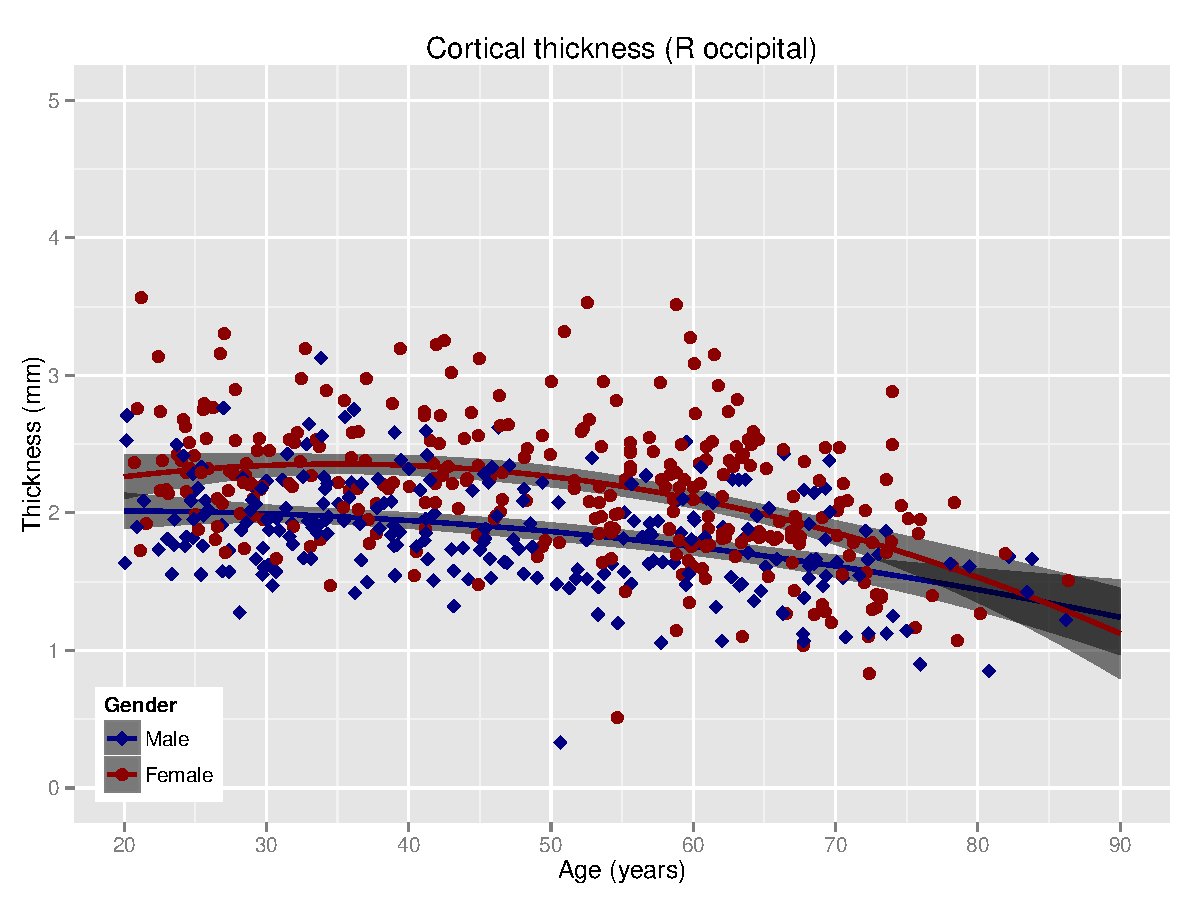
\includegraphics[width=51mm]{IXI_results/yylabel2_results.pdf} &
  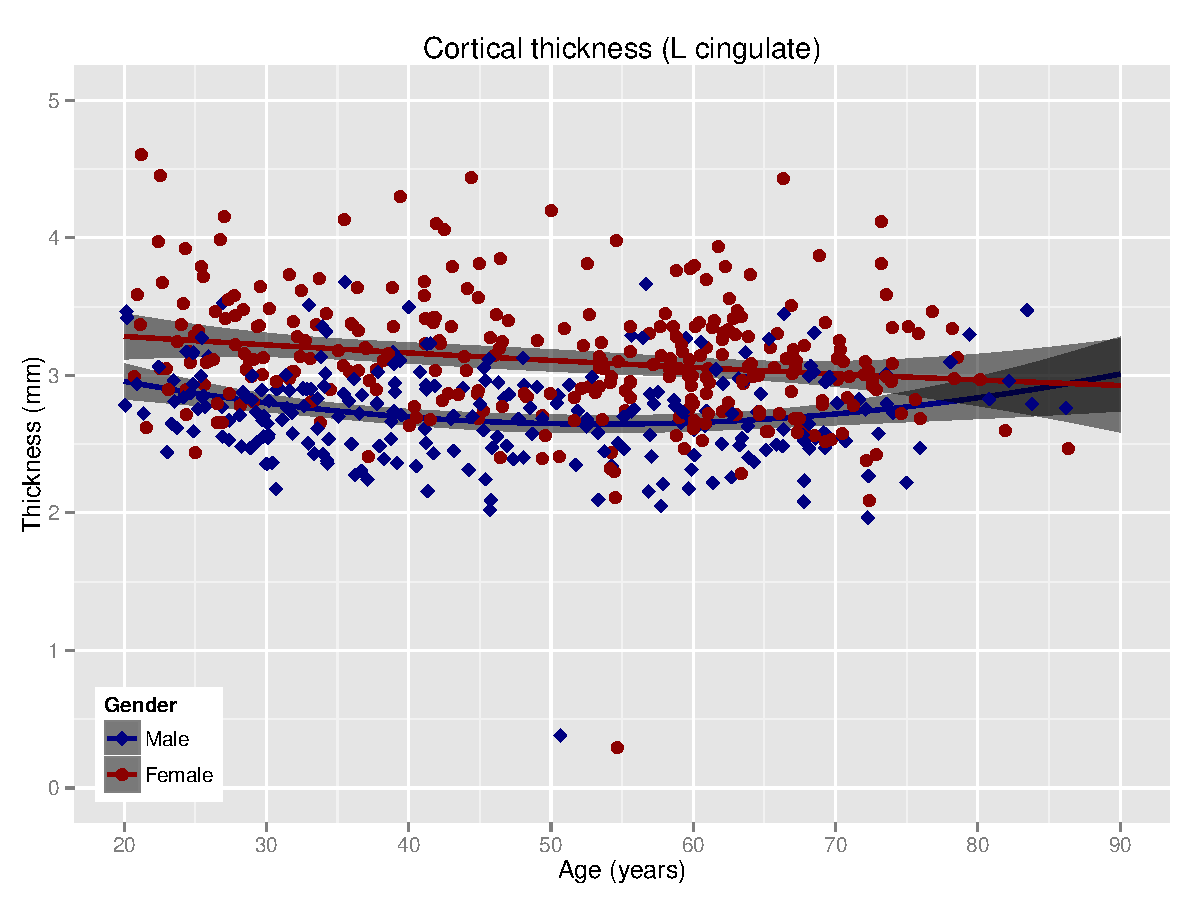
\includegraphics[width=51mm]{IXI_results/yylabel3_results.pdf} \\
  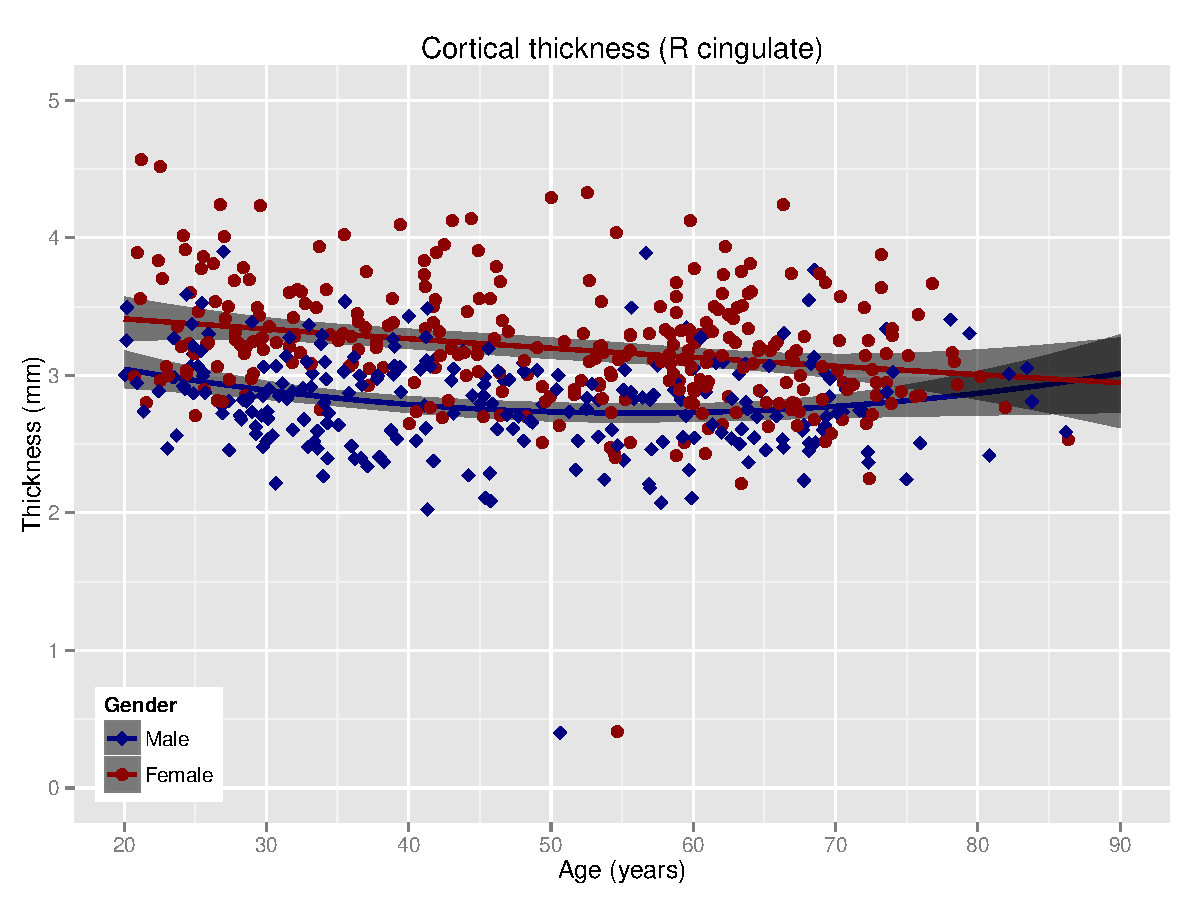
\includegraphics[width=51mm]{IXI_results/yylabel4_results.pdf} &
  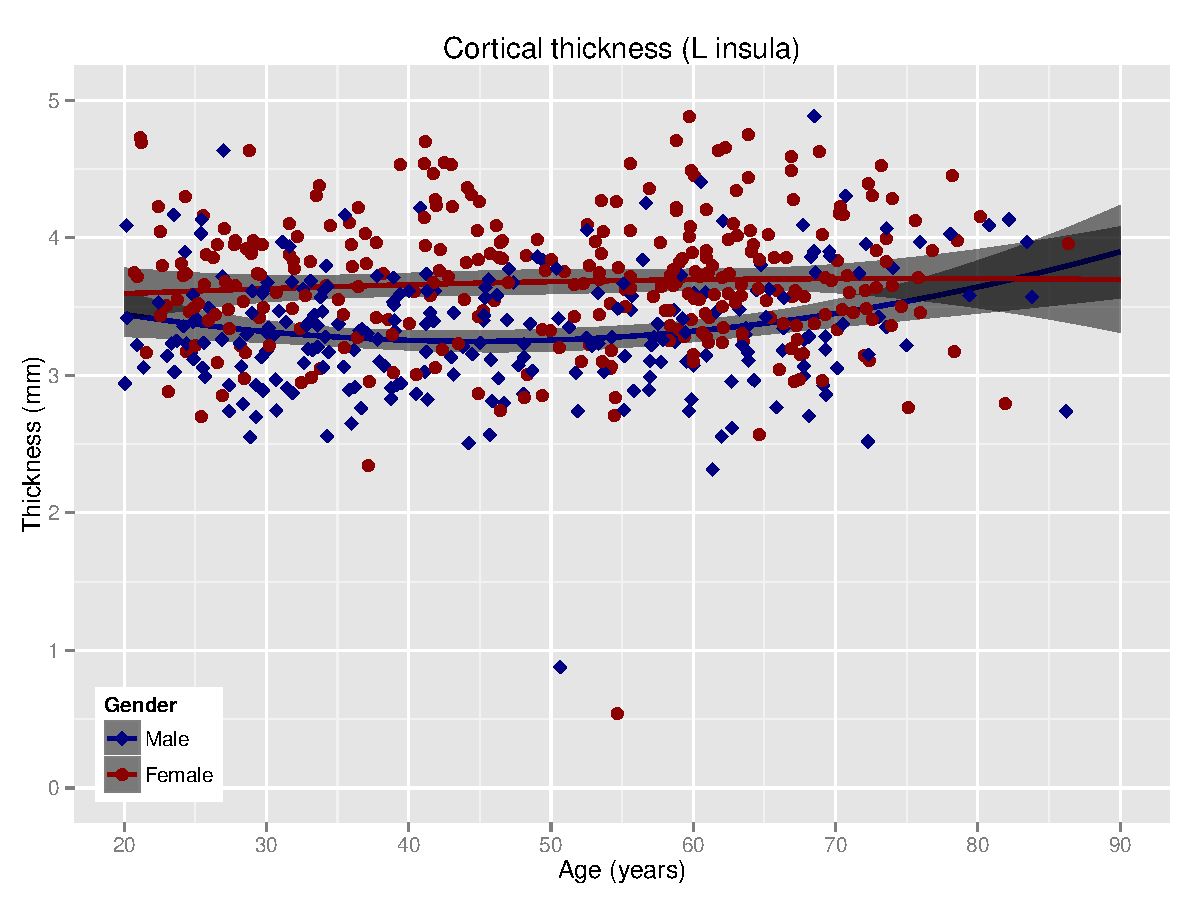
\includegraphics[width=51mm]{IXI_results/yylabel5_results.pdf} &
  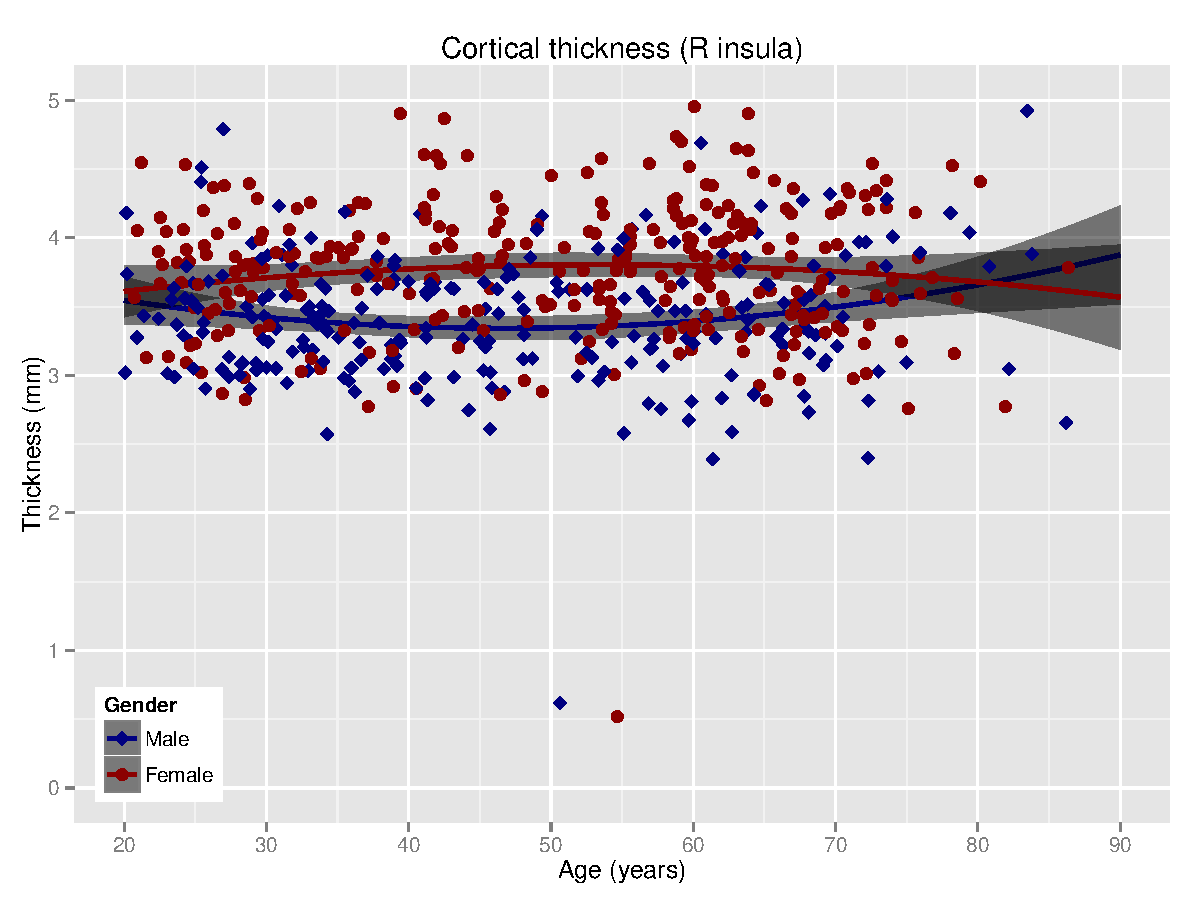
\includegraphics[width=51mm]{IXI_results/yylabel6_results.pdf} \\
  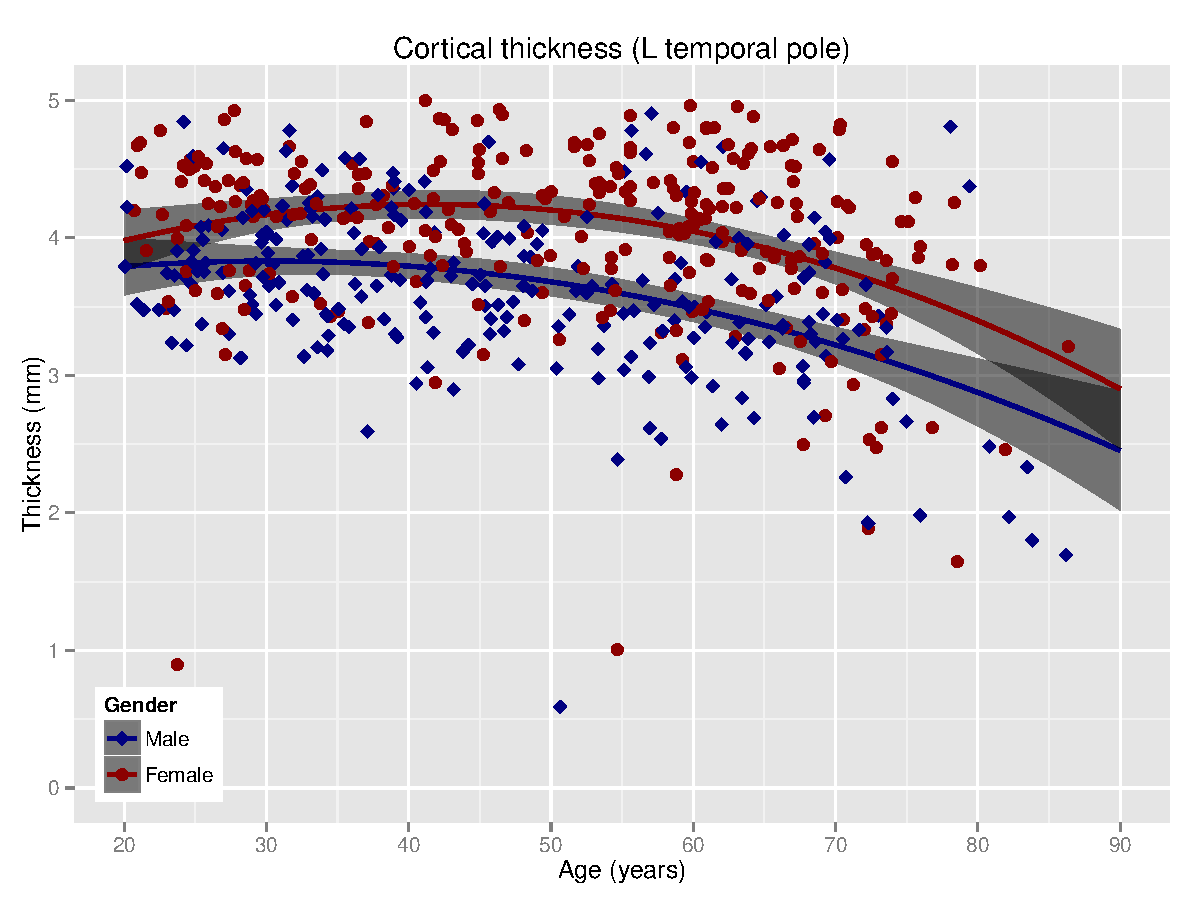
\includegraphics[width=51mm]{IXI_results/yylabel7_results.pdf} &
  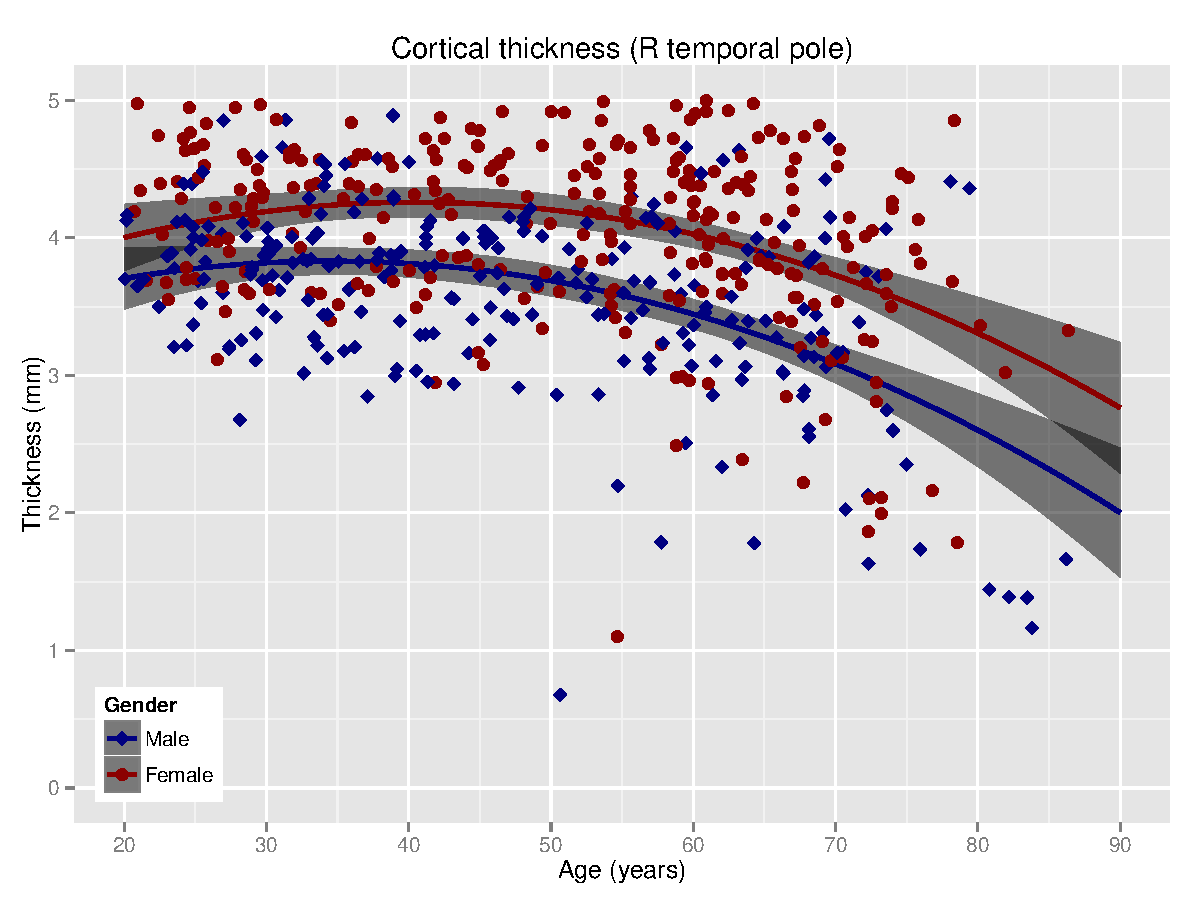
\includegraphics[width=51mm]{IXI_results/yylabel8_results.pdf} &
  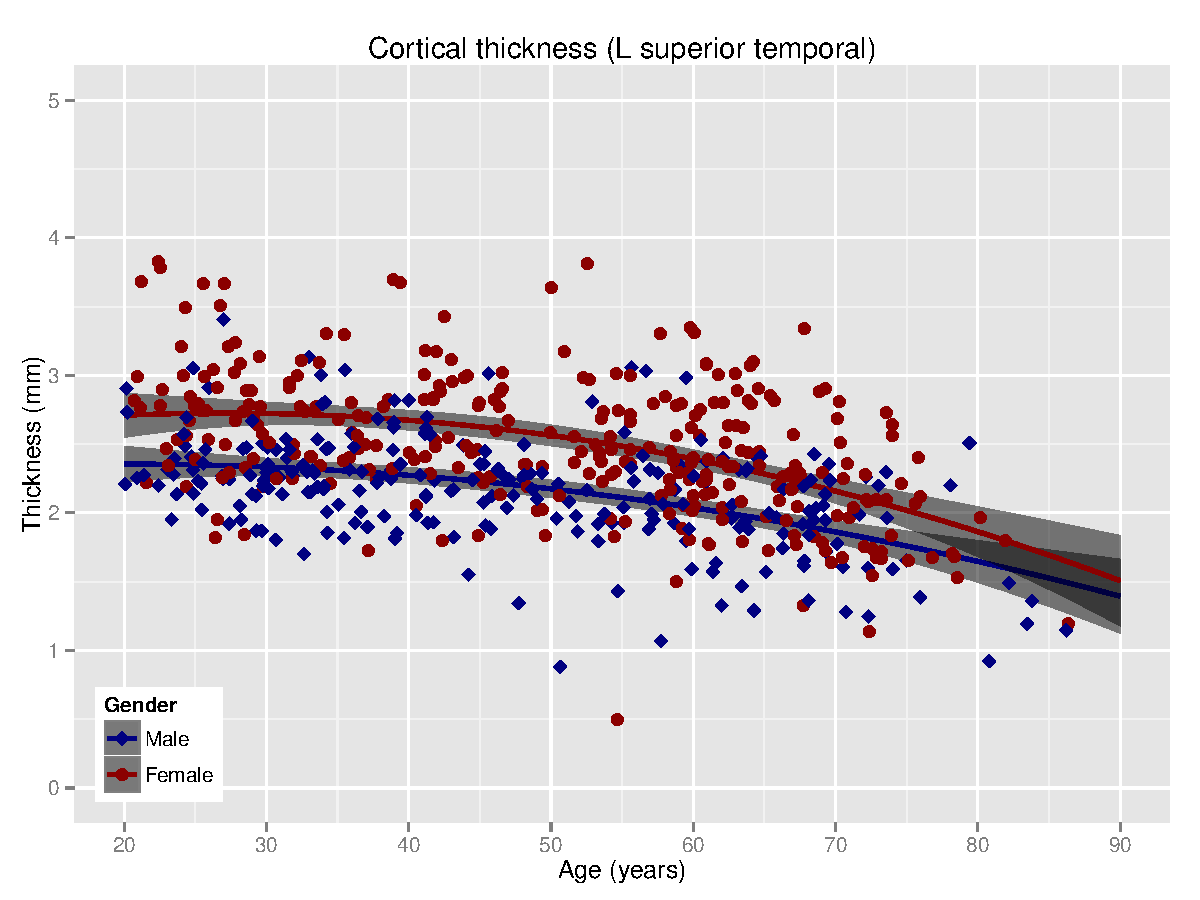
\includegraphics[width=51mm]{IXI_results/yylabel9_results.pdf} \\
  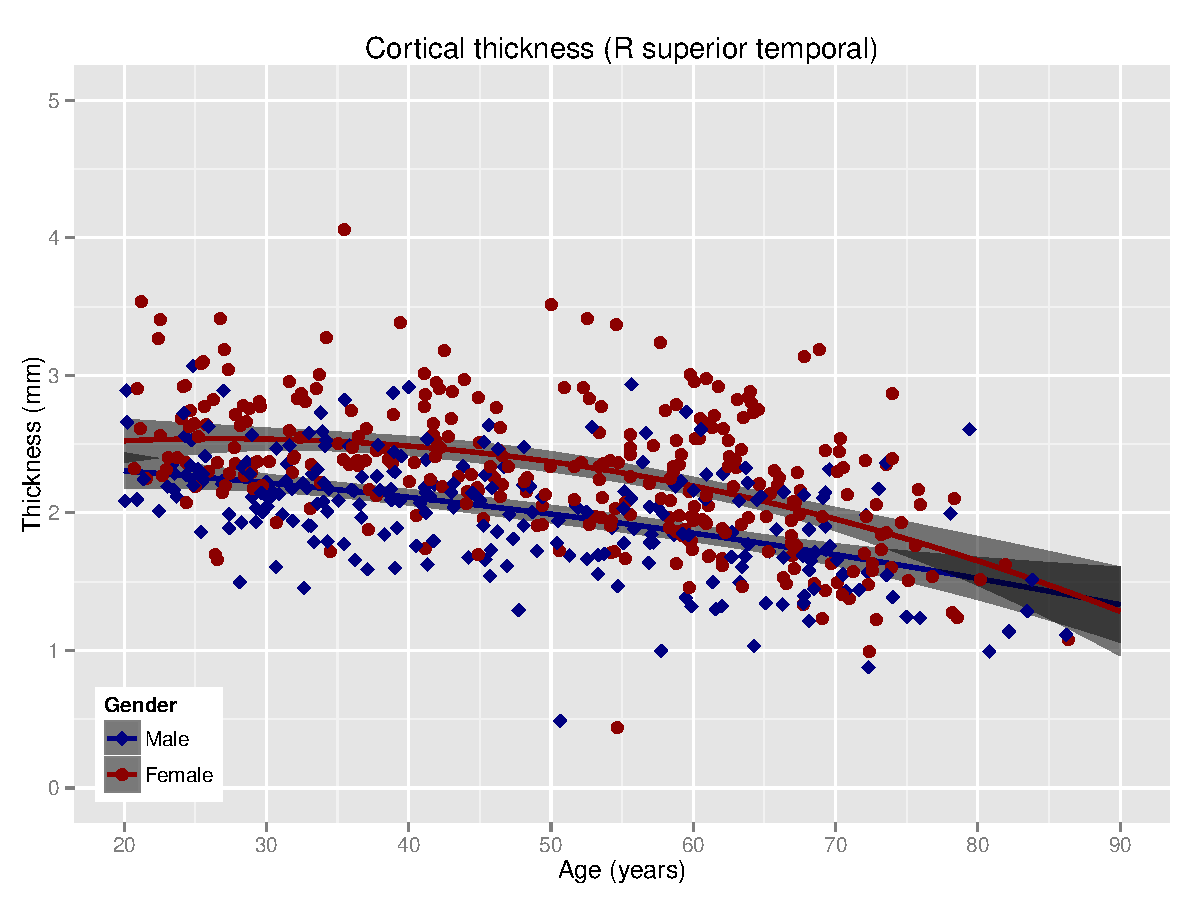
\includegraphics[width=51mm]{IXI_results/yylabel10_results.pdf} &
  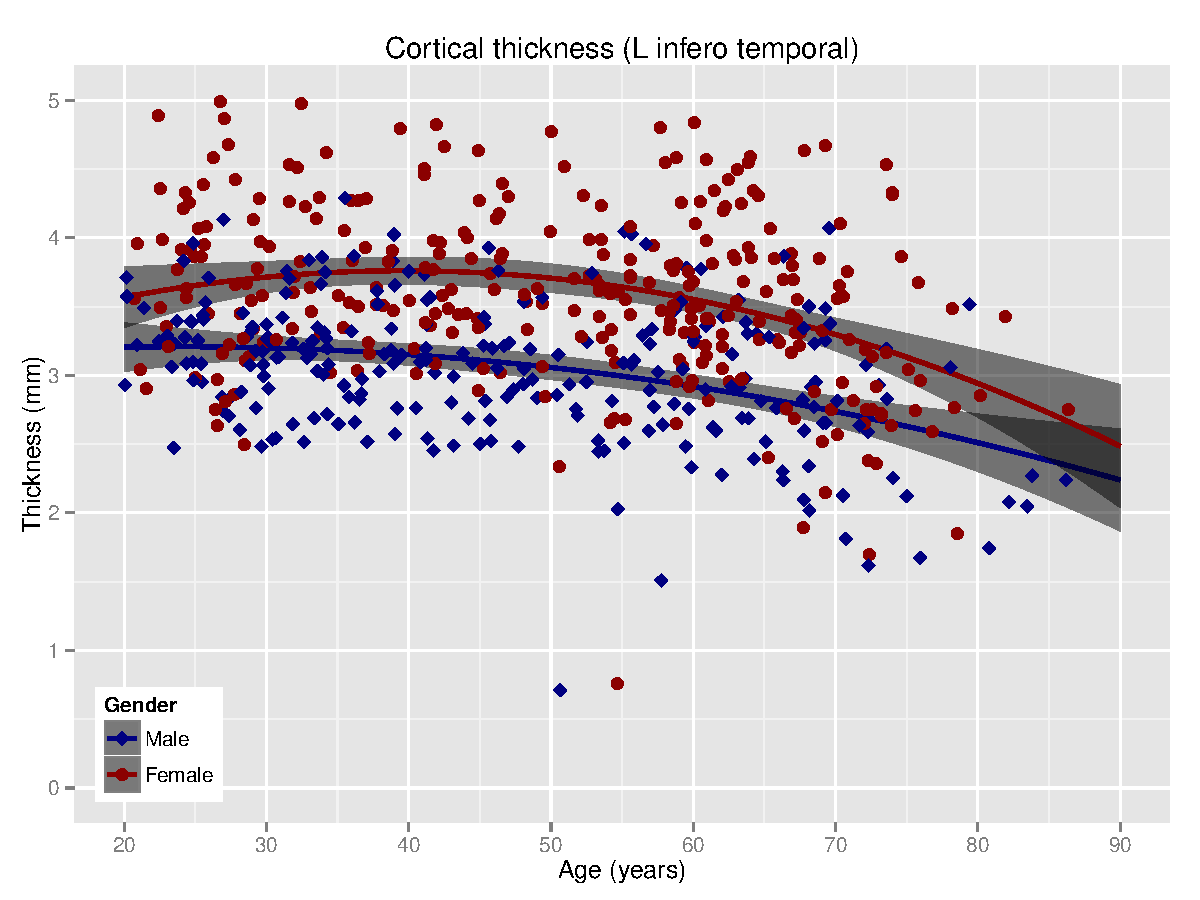
\includegraphics[width=51mm]{IXI_results/yylabel11_results.pdf} &
  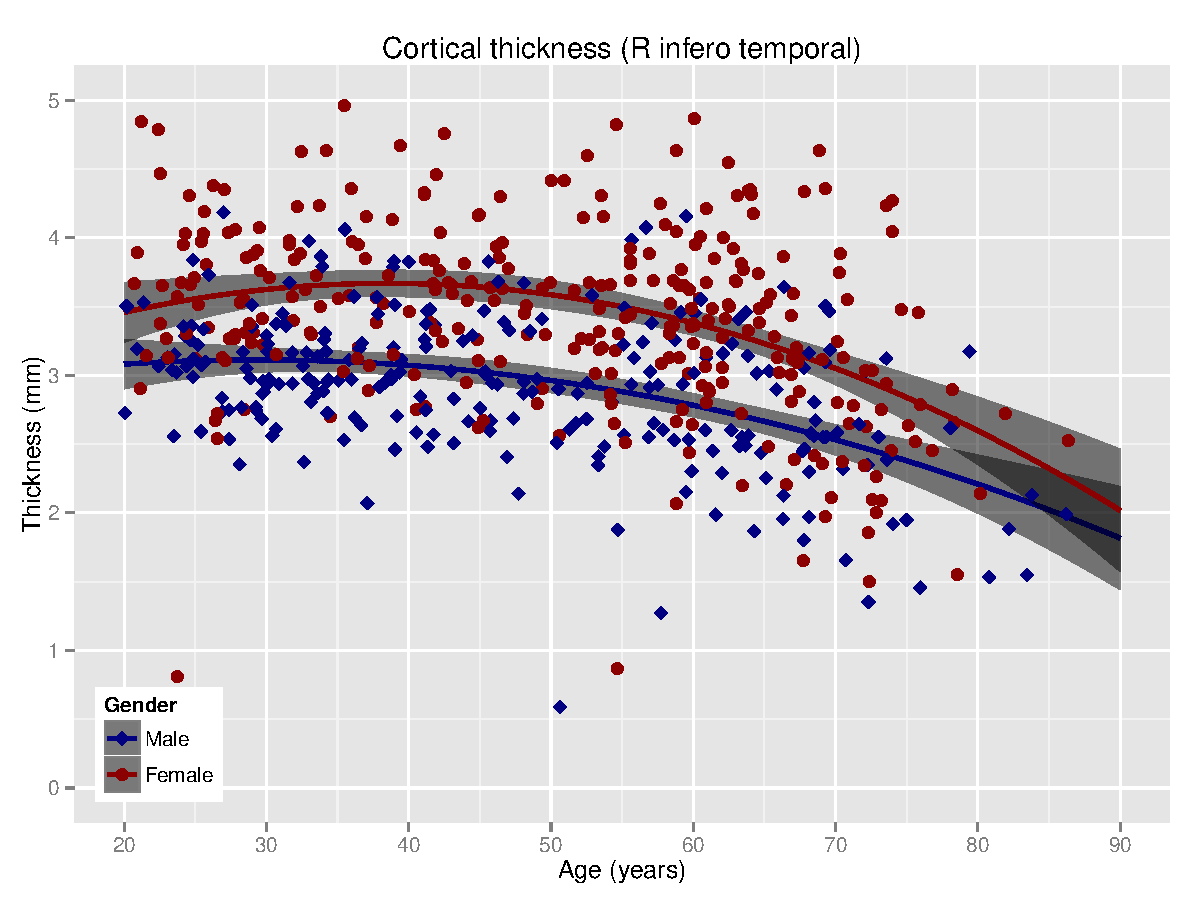
\includegraphics[width=51mm]{IXI_results/yylabel12_results.pdf} \\
  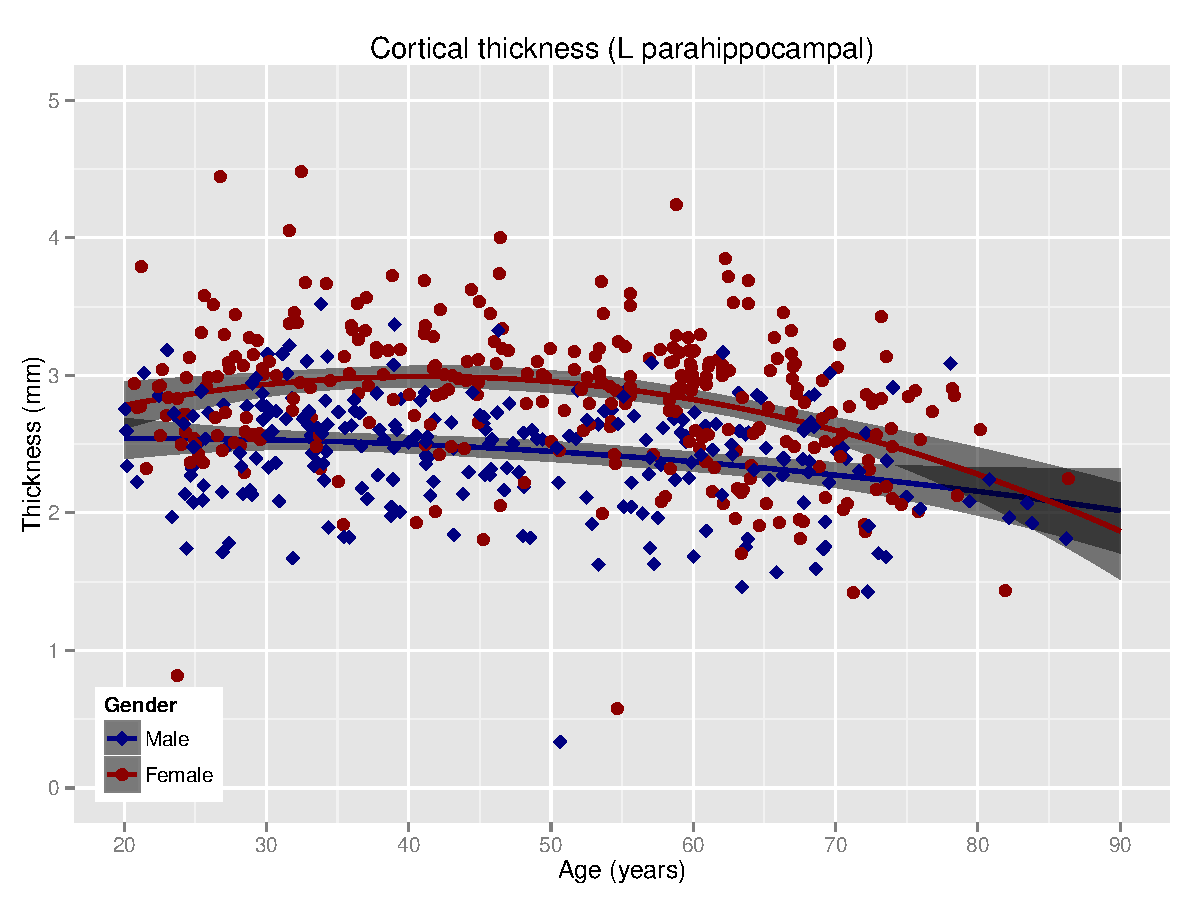
\includegraphics[width=51mm]{IXI_results/yylabel13_results.pdf} &
  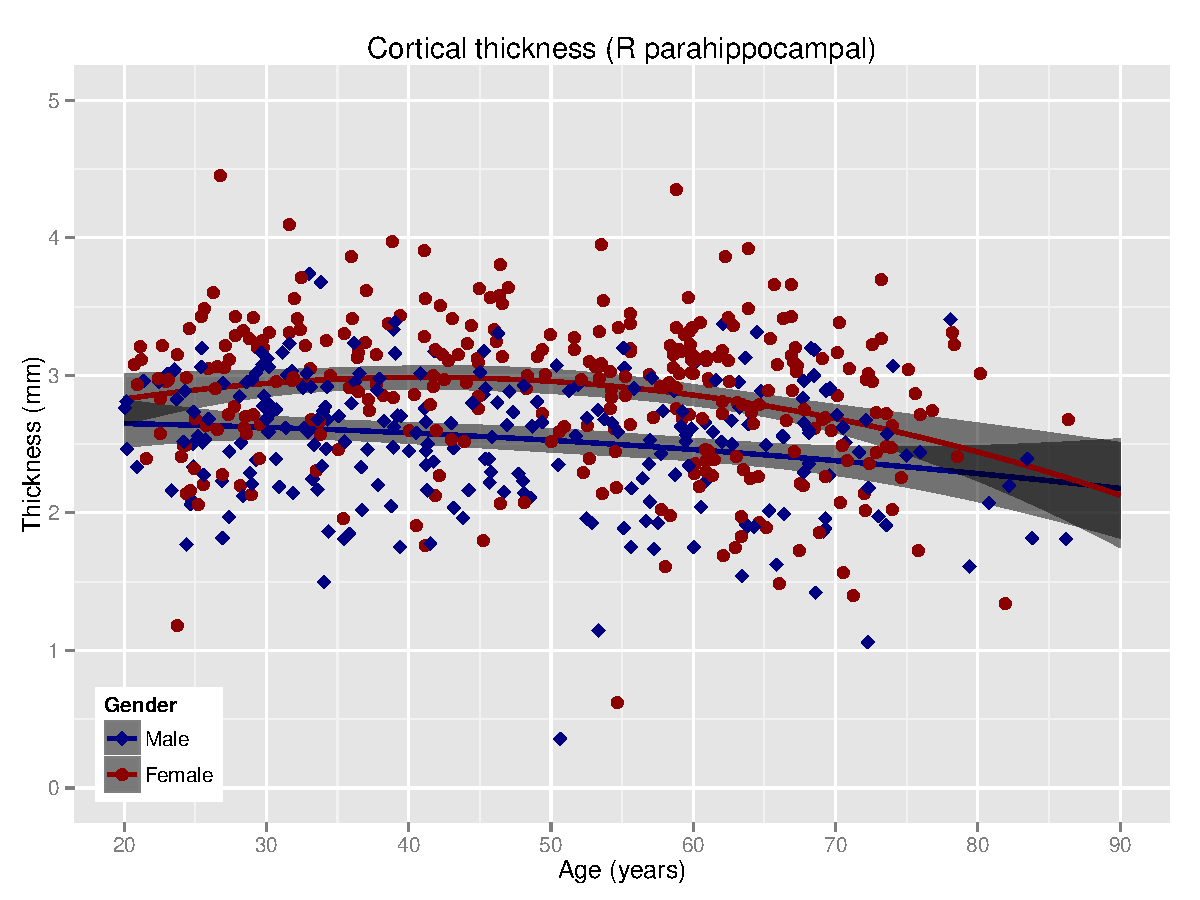
\includegraphics[width=51mm]{IXI_results/yylabel14_results.pdf} &
  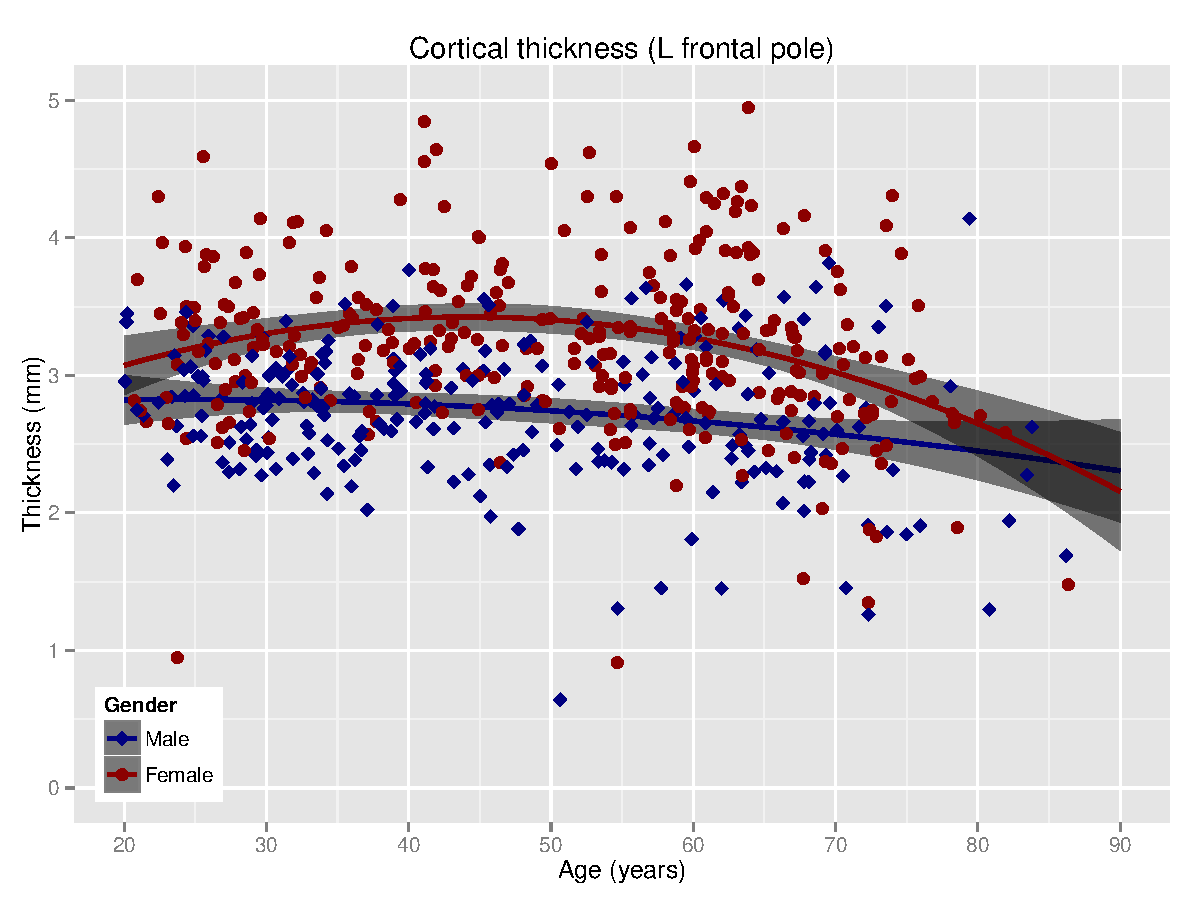
\includegraphics[width=51mm]{IXI_results/yylabel15_results.pdf} 
  \end{tabular}
  \caption{Cortical thickness results (age vs. thickness) from the IXI data set where
  each plot corresponds to one of the first 15 of 32 total cortical labels from the NIREP NA0 data set.  
  Thickness values have been normalized corresponding to the ratio of the individual 
  subject volume versus the total template volume.
  }
  \label{fig:nirep}
\end{figure}




%%%%%%%%%%%%%%%%%%%%%%%%%%%%%%%%%%%%%%%%%%%%%%%%%%%%%%%%%%%%%
\section{CONCLUSIONS} 

Given the numerous studies that have used cortical thickness for 
making neuroscientific inferences, it is of vital importance that
1) there be multiple, robust computational tools for extracting such
quantitative information and 2) that these tool sets be publicly 
available for validating research findings.  The Freesurfer package
has proven to be exemplary in this respect.  Our proposed work is
meant to compliment such packages as Freesurfer by providing a 
volume-based, well-vetted, open source resource for extracting 
cortical thickness maps in large studies.



%%%%%%%%%%%%%%%%%%%%%%%%%%%%%%%%%%%%%%%%%%%%%%%%%%%%%%%%%%%%%
%\acknowledgments     %>>>> equivalent to \section*{ACKNOWLEDGMENTS}       
% 
%This unnumbered section is used to identify those who have aided the authors in understanding or accomplishing the work presented and to acknowledge sources of funding.  

%%%%%%%%%%%%%%%%%%%%%%%%%%%%%%%%%%%%%%%%%%%%%%%%%%%%%%%%%%%%%
%%%%% References %%%%%

\bibliography{references}   %>>>> bibliography data in report.bib
\bibliographystyle{spiebib}   %>>>> makes bibtex use spiebib.bst

\end{document} 
